\documentclass[compress]{beamer}
\mode<presentation>
\setbeamercovered{transparent}
\usetheme{Warsaw}
%\useoutertheme{smoothtree}
\usepackage{multirow}
\usepackage[english]{babel}
\usepackage[latin1]{inputenc}
\usepackage{times}
\usepackage[T1]{fontenc}
\usepackage{xmpmulti}
\usepackage{multicol}
\usepackage{colortbl}
%\setbeamersize{text margin left=.25 in,text margin right=.25 in}
\setbeamersize{text margin left=.15 in,text margin right=.15 in}
\usepackage[authoryear]{natbib}
\usepackage{epstopdf}
\definecolor{antiquebrass}{rgb}{0.8, 0.58, 0.46}
\definecolor{babyblueeyes}{rgb}{0.63, 0.79, 0.95}
\definecolor{babyblue}{rgb}{0.54, 0.81, 0.94}
\definecolor{bistre}{rgb}{0.24, 0.17, 0.12}
\definecolor{brightlavender}{rgb}{0.75, 0.58, 0.89}
\definecolor{bulgarianrose}{rgb}{0.28, 0.02, 0.03}
\definecolor{slateblue}{rgb}{0.56, 0.74, 0.56}
\definecolor{cordovan}{rgb}{0.54, 0.25, 0.27}
\definecolor{darkbyzantium}{rgb}{0.36, 0.22, 0.33}
\setbeamercolor{structure}{fg=darkbyzantium!70, bg= black!60}
\usepackage{tikz}
\usetikzlibrary{shadows,calc}
\usetikzlibrary{shadows.blur}
\usetikzlibrary{shapes.symbols}
\usepackage{hyperref}
\usepackage{booktabs}
\usepackage{colortbl}
\usepackage{multirow}
%%%%%%%%% shaddow image %%%%%
% some parameters for customization
\def\shadowshift{3pt,-3pt}
\def\shadowradius{6pt}
\colorlet{innercolor}{black!60}
\colorlet{outercolor}{gray!05}
% this draws a shadow under a rectangle node
\newcommand\drawshadow[1]{
\begin{pgfonlayer}{shadow}
    \shade[outercolor,inner color=innercolor,outer color=outercolor] ($(#1.south west)+(\shadowshift)+(\shadowradius/2,\shadowradius/2)$) circle (\shadowradius);
    \shade[outercolor,inner color=innercolor,outer color=outercolor] ($(#1.north west)+(\shadowshift)+(\shadowradius/2,-\shadowradius/2)$) circle (\shadowradius);
    \shade[outercolor,inner color=innercolor,outer color=outercolor] ($(#1.south east)+(\shadowshift)+(-\shadowradius/2,\shadowradius/2)$) circle (\shadowradius);
    \shade[outercolor,inner color=innercolor,outer color=outercolor] ($(#1.north east)+(\shadowshift)+(-\shadowradius/2,-\shadowradius/2)$) circle (\shadowradius);
    \shade[top color=innercolor,bottom color=outercolor] ($(#1.south west)+(\shadowshift)+(\shadowradius/2,-\shadowradius/2)$) rectangle ($(#1.south east)+(\shadowshift)+(-\shadowradius/2,\shadowradius/2)$);
    \shade[left color=innercolor,right color=outercolor] ($(#1.south east)+(\shadowshift)+(-\shadowradius/2,\shadowradius/2)$) rectangle ($(#1.north east)+(\shadowshift)+(\shadowradius/2,-\shadowradius/2)$);
    \shade[bottom color=innercolor,top color=outercolor] ($(#1.north west)+(\shadowshift)+(\shadowradius/2,-\shadowradius/2)$) rectangle ($(#1.north east)+(\shadowshift)+(-\shadowradius/2,\shadowradius/2)$);
    \shade[outercolor,right color=innercolor,left color=outercolor] ($(#1.south west)+(\shadowshift)+(-\shadowradius/2,\shadowradius/2)$) rectangle ($(#1.north west)+(\shadowshift)+(\shadowradius/2,-\shadowradius/2)$);
    \shade[outercolor,right color=innercolor,left color=innercolor] ($(#1.north west)+(-\shadowradius/12,\shadowradius/12)$) rectangle ($(#1.south east)+(\shadowradius/12,-\shadowradius/12)$);%Frame
    \filldraw ($(#1.south west)+(\shadowshift)+(\shadowradius/2,\shadowradius/2)$) rectangle ($(#1.north east)+(\shadowshift)-(\shadowradius/2,\shadowradius/2)$);
\end{pgfonlayer}
}
% create a shadow layer, so that we don't need to worry about overdrawing other things
\pgfdeclarelayer{shadow} 
\pgfsetlayers{shadow,main}
% Define image shadow command
\newcommand\shadowimage[2][]{%
\begin{tikzpicture}
\node[anchor=south west,inner sep=0] (image) at (0,0) {\includegraphics[#1]{#2}};
\drawshadow{image}
\end{tikzpicture}}
\usepackage{calligra}

\DeclareMathOperator*{\argmax}{Arg\,max}
\DeclareMathOperator*{\argmin}{Arg\,min}
\newcommand{\norm}[1]{\left\Vert #1 \right\Vert }
\newcommand{\bbetaHat}{ \widehat{\bbeta}}
\newcommand{\bbetaLSE}{ \widehat{\bbeta}_{_{\text{LSE}}}}
\newcommand{\bbetaMLE}{ \widehat{\bbeta}_{_{\text{MLE}}}}
\newcommand{\sqBullet}[1]{  {\tiny \tiny \tiny \qBoxCol{#1!60}{ }} }
%***************
%\newtheorem{thm}{Theorem}
%\documentclass[noinfoline]{imsart}
%\usepackage{amsmath,amstext,amssymb}
%%\usepackage[top=1.5in, bottom=1.5in, left=1.2in, right=1.2in]{geometry}
%% settings
%%\pubyear{2005}
%%\volume{0}
%%\issue{0}
%%\firstpage{1}
%%\lastpage{8}
%\arxiv{arXiv:0000.0000}

%\startlocaldefs
%\numberwithin{equation}{section}
%\theoremstyle{plain}
%\newtheorem{thm}{Theorem}
%\endlocaldefs
\usepackage{lipsum} 
\usepackage{amsmath}
\usepackage{amssymb}
\usepackage{amsbsy} 
\usepackage{amsthm}
\usepackage{mathrsfs}
\usepackage{eufrak}
\usepackage{mathrsfs}
\usepackage{color}
\usepackage{verbatim}
\usepackage{graphicx}
\usepackage{bm}
\usepackage{enumerate}
\usepackage{epstopdf} 
\usepackage{natbib}
\usepackage{undertilde}
%\RequirePackage[colorlinks,citecolor=blue,urlcolor=blue]{hyperref}
%\usepackage{subfig}
\usepackage[final]{pdfpages}

\usepackage{algorithm}  %@subhajit
\usepackage{algpseudocode} %@subhajit
\usepackage{algorithmicx}     %@subhajit
\usepackage{undertilde}


\newcommand{\sphere}{{\mathbb{S}}}
\newcommand{\R}{\mathbb{R}}
\newcommand{\LatentV}{V}
\newcommand{\NC}{m}
\newcommand{\Priorf}{f_{prior}}
\newcommand{\FWOne}[2]{{{}_{1}\Psi _{1}\left[{\begin{matrix}(\frac{#1}{2},\frac{1}{2})\\(1,0)\end{matrix}};#2\right]} 
}


\newcommand{\HyPriorMu}{\thetabf}
\newcommand{\HyPriorAlpha}{\alpha}
\newcommand{\HyPriorBeta}{\beta}
\newcommand{\HyPriorK}{\zeta}
\newcommand{\Indicator}[1]{\mathbb{I}({#1 })}
\newcommand{\xb}{\bm{x}}
\newcommand{\bx}{\MakeVec{\bm{x}}}
\newcommand{\bX}{\bm{X}}
\newcommand{\by}{\MakeVec{\bm{y}}}
\newcommand{\bZ}{\bm{Z}}
\newcommand{\bF}{\bm{F}}
\newcommand{\btheta}{\MakeVec{{\bm{\theta}}}}
\newcommand{\Bpi}{\MakeVec{\boldsymbol{\pi}}}
\newcommand{\thetabf}{\MakeVec{\boldsymbol{\theta}}}
\newcommand{\Thetabf}{\boldsymbol{\Theta}}
\newcommand{\taubf}{\MakeVec{\boldsymbol{\tau}}}
\newcommand{\Tr}{Tr}


\newcommand{\bM}{\bm{M}}
\newcommand{\bD}{\MakeVec{\bm{D}}}
\newcommand{\bV}{\MakeVec{\bm{V}}}
\newcommand{\loglikmix}{\mathcal{L}_{\bM,\bD,\bV}}
\newcommand{\hypdc}{{}_0F_1\left(\frac{n}{2},\frac{D_c^2}{4}\right)}


\usepackage{xstring}
\usepackage[normalem]{ulem}
\definecolor{ultramarine}{RGB}{38,29,163}
\newcommand\PalDel[1]{{\color{red} {\sout{#1}}}}
\newcommand\Pal[1]{{\color{ultramarine}{#1}}}
\newcommand\PalRp[2]{\PalDel{#1} \Pal{#2}}
\newcommand\PalCmnt[1]{{\color{ultramarine} {[[[***PAL:  #1 ***]]]}}}

\newcommand{\qedwhite}{\hfill \ensuremath{\Box}}
\newcommand{\SpaceD}{\mathcal{S}_p}
\newcommand{\SpaceM}{\widetilde{\mathcal{V}}_{n,p}}
\newcommand{\SpaceV}{\mathcal{V}_{p,p}}
\newcommand{\SpaceF}{\mathbb{R}^{n,p}}
\newcommand{\StiefelS}{\mathcal{V}_{n,p}}
\newcommand{\SpacePi}{\mathbb{S}_{\pi}}
\newcommand{\ML}{{\cal{ML}}}
\newcommand{\ProdSpace}{\boldsymbol{\Theta}}
\newcommand{\ThetaAndPi}{\Xi}
\newcommand{\ClassML}{\mathcal{C}_{\ML}}


\newcommand{\balpha}{\MakeVec{\bm{\alpha}}}
\newcommand{\bbeta}{\MakeVec{\bm{\beta}}}
\newcommand{\bEta}{\bm{\eta}}
\newcommand{\bd}{{\utilde{\bm{d}}}}
\newcommand{\BoEta}{{\utilde{\boldsymbol{\eta}}}}
%\newtheorem{theorem}{Theorem}[section]
%\newtheorem{theorem}{Theorem}
%\newtheorem{lemma}{Lemma}
%\newtheorem{result}{Result}
\newtheorem{defn}{Definition}
\newcommand{\pdv}[2][]{\frac{\partial#1}{\partial#2}}
\newcommand{\pdvtwo}[2][]{\frac{\partial^2#1}{{\partial#2}^2}}


\newcommand{\mubf}{\boldsymbol{\mu}}
\newcommand{\sumI}{ \sum_{i=1}^{n}}
\newcommand{\Ybar}{{\overline{Y}}}

\newcommand{\Expectation}[1]{\mathbb{E}{[#1]}}
\newcommand{\priorXzero}{\Psi}
\newcommand{\iMat}{\mathbf{I}_{p}}

% 
% \newtheorem{thm}{Theorem}[section]
% \newtheorem{cor}[thm]{Corollary}
% \newtheorem{lem}[thm]{Lemma}
%\newtheorem{proposition}{Proposition}

%\newtheorem{theorem}{Theorem}[chapter]%To link the theorem to each chapter uncomment the chapter option
%\newtheorem{lemma}{Lemma}%[theorem]% To link each lemma to a theorem uncomment the theorem option
%\newtheorem{corollary}{Corollary}%[theorem]% To link each corollary to a theorem uncomment the theorem option
% to link a corollary to a chapter change the theorem option to chapter
%\newtheorem{definition}{Definition}%[chapter] %the same is true for both definitions and assumptions
\newtheorem{assumption}{Assumption}%[chapter] %
%\newtheorem{proposition}{Proposition}[chapter]
%\newtheorem{fact}{Fact} %%% added by @subho
\newcommand{\StrongNBD}[2]{S_{#1}{#2}}
\newcommand{\bpi} {\boldsymbol{\pi}}
\newcommand{\bphi} {\boldsymbol{\phi}}
\newcommand{\bb}[1]{\boldsymbol{#1}}
% Definitions of handy macros can go here

\newcommand{\normtwo}[1]{{\left\lVert#1\right\rVert}_2}

\newcommand{\dataset}{{\cal D}}
\newcommand{\fracpartial}[2]{\frac{\partial #1}{\partial  #2}}
\newcommand{\Lesbegue}[1]{\mu_{\btheta_{#1},\bpi_{#1}}}
\newcommand{\fthetapi}[1]{f_{\btheta_{#1},\bpi_{#1}}}
% Heading arguments are {volume}{year}{pages}{submitted}{published}{author-full-names}
\newcommand{\doublehat}[1]{%
    \settoheight{\dhatheight}{\ensuremath{\widehat{#1}}}%
    \addtolength{\dhatheight}{-0.35ex}%
    \widehat{\vphantom{\rule{2pt}{\dhatheight}}%
    \smash{\hspace{-0.5mm}\widehat{#1}}}}

\newcommand{\hyp}{{}_0F_1\left(\frac{n}{2},\frac{D^2}{4}\right)}
\newcommand{\hypinline}{{}_0F_1\left({n}/{2},{D^2}/{4}\right)}

\newcommand{\partialhyp}[1]{\frac{\partial}{\partial\,{d_{#1}}}\,\left[\hyp\right]}

\newcommand{\fracProbZ}[1]{\frac{\langle Z_{ic} \rangle \, #1}{\sum_{i=1}^{N} \langle Z_{ic}\rangle  } }
\newcommand{\EmVar}[1]{\widetilde{#1}^{(c)}}

\newcommand{\IMDY}{{\it{CCPD}}}
\newcommand{\JMDY}{{\it{JCPD}}}

\newcommand{\DYlang}{\frac{\exp(\nu\,\bEta^T\bd)}{{\left[{}_0F_1\left(\frac{n}{2},\frac{D^2}{4}\right)\right]}^{\nu}}}

\newcommand{\logDYlang}{\nu\,\bEta^T\bd - \nu\,\log\left({}_0F_1\left(\frac{n}{2},\frac{D^2}{4}\right)\right)}

\newcommand{\lhyp}{\log\left({}_0F_1\left(\frac{n}{2},\frac{D^2}{4}\right)\right)}

%\jmlrheading{1}{2000}{1-48}{4/00}{10/00}{SS \& JH \& AB}

% Short headings should be running head and authors last names

%\ShortHeadings{BDP and cIBP}{SS \& JH \& AB}
%\firstpageno{1}

\newcommand{\diam}[1]{{{#1}^{\ast}}}

%%% coloring option %%%
\definecolor{auburn}{rgb}{0.53, 0.1, 0.5}
\newcommand{\sss}{\color{auburn}}  %%% for Subhajit
\newcommand{\sse}{\color{black}}
\newcommand{\attn}{\color{red}}
\newcommand{\rms}{\color{magenta}}  %%% for Riten
\newcommand{\rme}{\color{black}}
\newcommand{\MLDensity}{f_{\ML}}
\setlength{\parindent}{0cm}
\newcommand{\posterior}

\newcommand{\variableX}{\bd}
\newcommand{\funch}{\mathfrak{h}}
\newcommand{\IndVzero}[1]{\mathbb{I}({X\in \mathcal{V}^{#1}_0})}
\newcommand{\Rnp}{\mathbb{R}^{n \times p}}
\newcommand{\Rpp}{\mathbb{R}^{p \times p}}
\newcommand{\vecnorm}[1]{\lVert #1\rVert}

\newcommand{\etapsiD}{\eta_{\priorXzero}}
\newcommand{\BoEtapsiD}{\BoEta_{\priorXzero}}

\newcommand{\DMp}{\mathcal{D}^{p \times p}}
\newcommand{\Rplus}{\mathbb{R}_{+}}
\newcommand{\prodMeasure}{\Upsilon}

\newcommand{\m}{{\bf m_{\BoEta}}} 
\newcommand{\SetWithMode}{\mathcal{S}}
\newcommand{\SetWithModePrime}{\mathcal{S}}
\newcommand{\TargetComp}{\mathcal{S}^{\star}}

\newcommand{\ConstCondDen}{K_{\nu, \BoEta}} 

\newcommand{\hyparam}[2]{
    \IfEqCase{#1}{
        {M}{\xi^{#2}_c}
        {V}{\gamma^{#2}_c}%
        
    }
  }
\newcommand{\threepartdef}[6]
{
	\left\{
		\begin{array}{lll}
			#1 & \mbox{if } #2 \\
			#3 & \mbox{if } #4 \\
			#5 & \mbox{if } #6
		\end{array}
	\right.
}

\def\bv{\color{blue}}
\def\ev{\color{black}}
\newcommand{\bch}{\bv }
\newcommand{\ech}{\ev\normalsize}
%\newcommand{\MakeVec}[1]{{\utilde{\bf #1}}}
\newcommand \Measure[2][]{%
  \ifstrempty{#1}{
  \IfEqCase{#2}{
        {M}{\mu}%
        {D}{\mu_1}%
        {V}{\mu_2}
        {X}{\mu}
   }  
  }{
  \IfEqCase{#1}{
  {1}{
   \IfEqCase{#2}{
        {M}{d\mu(M)}%
        {D}{d\mu_1(\bd)}%
        {V}{d\mu_2(V)}
        {X}{d\mu(X)}
        {Y}{d\mu(Y)}
        {MDV} {d\mu(M)\; d\mu_1(\bd) \;d\mu_2(V) }
        }
   } 
   {2}{
   \IfEqCase{#2}{
         {M}{d\mu(M^{\ast})}%
        {D}{d\mu_1(\bd^{\ast})}%
        {V}{d\mu_2(V^{\ast})}
        {X}{d\mu(X^{\ast})}
        }
   }
   {3}{
   \IfEqCase{#2}{
         {M}{\mu(dM^{\star})}%
        {D}{\mu_2(d\bd^{\star})}%
        {V}{\mu_1(dV^{\star})}
        {X}{\mu(X^{\star})}
        }
   }   
   
   } 
  }%
}
  \newcommand{\VONF}{\text{VonMisesFisher}}
\newcommand{\MPGalpha}{\alpha}
\newcommand{\MPGnu}{\nu}
\newcommand{\MPG}{MPG }
\newcommand{\ybin}{y^{(\text{bin})}}


%\newcommand{\abs}[1]{\left \vert  #1  \right\vert  }
\usepackage{caption}
\usepackage{subcaption}

%%%%%%%%%%%%%%%%%%%%%%%%%%%
\newcommand{\IEHC}{\text{IEHC}}







\newcommand \Th[1]{%
  \IfEqCase{#1}{
        {1}{ 1^{\text{st}}}%
        {2}{2^{\text{nd}}}%
        {3}{3^{\text{rd}}}%
  }[{#1}^{\text{th}}]
}
  
  
   \newcommand{\augV}{\text{aux}}
  
  
  
  
  \newcommand{\CDE}{\text{PL}}
\newcommand{\CDEsigma}{\sigma}
\newcommand{\CDEepsilon}{\SVepsilon}
\newcommand{\CDEmu}{\mu}
 % \newcommand{\SVepsilon}{\varepsilon}
  \newcommand{\SVepsilon}{\delta}
 \newcommand{\abs}[1]{\left\lvert{#1}\right \rvert }
 
 
\newcommand{\CPDX }{\text{CPDX}}
\newcommand{\CPDXPar}{\vartheta}
\newcommand{\K}{\mathcal{K}}



\newcommand{\lossFunctionOne}[1]{ \left\{ \abs{ ( \abs{#1}-\SVepsilon)}  + ( \abs{#1}-\SVepsilon)\right\} }

\newcommand{\lossFunctionAlt}[1]{ \abs{  #1-\SVepsilon}  + \abs{ #1+\SVepsilon}-2\SVepsilon }

\newcommand{\lossFunctionAltOne}[1]{   \lossFunctionAlt{ \frac{\left(#1\right)}{\sigma}}}

\newcommand{\lossFunction}[1]{ \left\{ \abs{ \left( \frac{\abs{#1}}{\sigma}-\SVepsilon\right)}  + \left( \frac{\abs{#1}}{\sigma}-\SVepsilon\right)\right\} }
\newcommand{  \Likelihood}{\mathcal{L}}
%\newcommand{\Onebf}{\bf 1}
\newcommand{\Onebf}{{\bf \utilde{1}_{n}}}





\newcommand{\InvGamma}{\text{InvGamma}}
\newcommand{\PriorSigmaAlpha}{a}
\newcommand{\PriorSigmaBeta}{b}
\newcommand{\PriorBetaMean}{\mubf_{_{\bbeta}}}
\newcommand{\PriorBetaVar}{\Sigma_{_{\bbeta}}  }
\newcommand{\mvnormPdf}[4]{\frac{1}{ \left({2\pi}\right)^{\frac{#4}{2}} \sqrt{\vert{#3}\vert}}{\exp\left[ - \frac{1}{2}(#1- #2)^T {#3}^{-1} (#1- #2)\right]}      }
\newcommand{\InvGammaPdf}[3]{ \frac{(#1)^{-#2+1}}{\Gamma\left( #2\right) } \exp\left[ -\frac{{#3}}{{#1}} \right] }

 \newcommand{\byTilde}{\tilde{\by}}
 
 \newcommand{\TrfSigma}{\varsigma}
 \newcommand{ \Normal}{\text{Normal}}
 \newcommand{\GlobalPar}{\tau}
\newcommand{\LocalPar}{\psi}
\usepackage{xcolor}
\usepackage{xparse}
\definecolor{lightGray}{gray}{0.95}
\definecolor{lightGrayOne}{gray}{0.9}
\definecolor{lightBlueOne}{RGB}{204, 255, 255}
\definecolor{lightBlueTwo}{RGB}{204, 238, 255}
\definecolor{lightBlueThree}{RGB}{204, 204, 255}
\definecolor{AltBlue}{RGB}{119,14,161}
\definecolor{Orchid}{RGB}{186,85,211}

\definecolor{BGBlue}{RGB}{220,221,252}
\definecolor{BGBlueOne}{RGB}{204,229,255}

\definecolor{DarkGreenOne}{RGB}{34,139,34}

\definecolor{BGGreen}{RGB}{240,243,245}
\definecolor{lightGreenOne}{RGB}{179, 255, 179}
\definecolor{lightGreenTwo}{RGB}{198, 255, 179}
\definecolor{lightGreenThree}{RGB}{243, 255, 230}
\definecolor{AltGreen}{RGB}{193, 240, 240}

\definecolor{BOGreen}{RGB}{180,0,0}
\definecolor{BGGreenOne}{RGB}{220,250,220}

\definecolor{lightBrownOne}{RGB}{255, 221, 204}
\definecolor{lightBrownTwo}{RGB}{255, 229, 204}
\definecolor{lightBrownThree}{RGB}{242, 217, 230}


\definecolor{HLTGreen}{RGB}{230,244,215}
\definecolor{ExcBrown}{RGB}{153,0,0}
\definecolor{ExcBGBrown}{RGB}{255,204,204}
\definecolor{BGYellowOne}{RGB}{255,235,208}
\definecolor{BGPink}{RGB}{255,215,240}

\newcommand{\MakeVec}[1]{{\utilde{\bf #1}}}

\NewDocumentCommand{\MCOption}{O{1.75in} m}{
\TextInBoxTwo[BGPink]{ #1 } {\TextInBoxTwo[white]{.1 in }{ \quad}\HLT{#2}}
}

 \NewDocumentCommand{\ThreeChoices}{O{Do not Know}O{Not confident}O{Confident}}{
\MCOption{#1} \MCOption{#2} \MCOption{#3}
}
 
\NewDocumentCommand{\OneBlock}{ O{HLTGreen} m m }{\colorbox{#1}{\begin{minipage}{#2} $ #3$ \end{minipage}}}

\NewDocumentCommand{\HLT}{ O{HLTGreen} m }{\colorbox{#1}{#2}}
%\NewDocumentCommand{\HLTEQ}{ O{HLTGreen} m }{\colorbox{#1}{$#2$}}
\NewDocumentCommand{\HLTEQ}{ O{white} m }{\colorbox{#1}{$#2$}}

%\newcommand{\HLT}[1]{\colorbox{HLTGreen}{#1}}
\newcommand{\DEHLT}[1]{\colorbox{lightGrayOne}{\color{white} #1}}

\newcommand{\TextInBoxOne}[2]{  {\fcolorbox{white}{lightGrayOne}{\begin{minipage}{#1}  #2 \end{minipage}}}}


\NewDocumentCommand{\TextInBoxTwo}{ O{lightGrayOne} m m } {{\fcolorbox{white}{#1}{\begin{minipage}{#2} { #3} \end{minipage}}}}


\newcommand{\TextInBox}[2]{  {\fcolorbox{BGGreen}{BGGreen}{\begin{minipage}{#1}  #2 \end{minipage}}}}
\newcommand{\TextInBoxCol}[2]{
\fcolorbox{BGBlue}{BGBlue}{%
\begin{minipage}{#1}
 {\color{AltBlue} #2}
\end{minipage}}%
}

\NewDocumentCommand{\TxtBnd}{ O{lightBrownOne} m m } {{\fcolorbox{white}{#1}{\begin{minipage}{#2} { #3} \end{minipage}}}}


\newcommand{\BandInTopBox}[2]{
\fcolorbox{AltBlue}{AltBlue}{%
\begin{minipage}{#1}{ {\color{white}  #2 \hspace{.1in}} }
\end{minipage}}%
}


\newcommand{\TextInBoxThm}[2]{
\fcolorbox{AltBlue}{lightGray}{%
\begin{minipage}{#1}
 {\color{black} #2}
\end{minipage}}%
}

\newcommand{\TextInBoxThmOne}[2]{
\fcolorbox{BGBlue}{BGBlueOne}{%
\begin{minipage}{#1}
 {\color{AltBlue} #2}
\end{minipage}}%
}

\newcommand{\TextInBoxLem}[2]{
\fcolorbox{BGBlue}{lightGray}{%
\begin{minipage}{#1}
 {\color{black} #2}
\end{minipage}}%
}



\newcommand{\TextInBoxLemOne}[2]{
\vspace{.02 in}
\noindent
\fcolorbox{BGBlue}{BGBlue}{%
\begin{minipage}{#1}
 {\color{AltBlue} #2}
\end{minipage}}%
}



\newcommand{\DefBox}[1]{
%\vspace{.1 in}
\noindent
\TextInBoxLem{4.5 in }{
\BandInTopBox{4.4 in }{}
\TextInBoxLemOne{4.4 in }{
#1
}}}





\newcommand{\DefBoxOne}[2]{
%\vspace{.1 in}
\noindent
\TextInBoxLem{4.5 in }{
\BandInTopBox{4.4 in }{#1}
\TextInBoxLemOne{4.4 in }{
#2
}}}


\newcommand{\ThmBox}[2]{
\noindent
\TextInBoxThm{4.4 in }{
\TextInBoxThmOne{4.4 in }{
#1}
#2}
}

\newcommand{\LemBox}[2]{
\noindent
\TextInBoxLem{4.5 in }{
\TextInBoxLemOne{4.4 in }{
#1}
#2}
}

\newcommand{\PropBox}[2]{
\vspace{.1 in}
\noindent
\TextInBoxLem{4.5 in }{
\TextInBoxLemOne{4.4 in }{
#1}
#2}
}




\newcommand{\TextInBoxExc}[2]{
\noindent
\fcolorbox{white}{BGGreenOne}{%
\begin{minipage}{#1}
 {\color{black} #2}
\end{minipage}}%
}


\newcommand{\TextInBoxExample}[2]{
\noindent
\fcolorbox{white}{BGPink}{%
\begin{minipage}{#1}
 {\color{black} #2}
\end{minipage}}%
}


\newcommand{\ExerciseBox}[1]{
\noindent
%\TextInBoxLem{6 in }{
\TextInBoxExc{6 in }{
#1}
%#2}
}


\newcommand{\ExampleBox}[1]{
\noindent
%\TextInBoxLem{6 in }{
\TextInBoxExample{6 in }{
#1}
%#2}
}

\NewDocumentCommand{\CommentBox}{ O{BGBlue}  m }{
\TextInBoxLem{5.5in }{
{\bf Comment:}\\
\TextInBoxLemOne{5.4 in }{
#2}}
}



\newcommand{\HLTY}[1]{\HLTEQ[yellow]{#1}}
\newcommand{\HLTW}[1]{\HLTEQ[white]{#1}}



\newcommand{\qBox}[1]{
  \begin{tikzpicture}
\node[draw=none,shade,
      top color=lightGrayOne,
      bottom color=lightGray,
      rounded corners=2pt,
      blur shadow={shadow blur steps=5}
    ] at (0,0) {    \noindent 
\fcolorbox{white}{BGBlue}{%
\begin{minipage}{4.55 in}
 {\color{black} {
 #1}}
\end{minipage}  }%
 };
 
    \end{tikzpicture}
}
 
 


 

\newcommand{\qBoxCol}[2]{
  \begin{tikzpicture}
\node[draw=none,shade,
      top color=lightGrayOne,
      bottom color=lightGray,
      rounded corners=2pt,
      blur shadow={shadow blur steps=5}
    ] at (0,0) {    \noindent
\fcolorbox{white}{#1}{%
%\begin{minipage}{4.55 in}
\begin{minipage}{4.55 in}
 {
 \color{black} {
 #2}}
\end{minipage}  }%
 };
 
    \end{tikzpicture}
}
  
  
  
  
  
  

\NewDocumentCommand{\qBrd}{O{4.55 in} m m}{
  \begin{tikzpicture}
\node[draw=none,shade,
      top color=#2,
      bottom color=#2,
      rounded corners=2pt,
      blur shadow={shadow blur steps=5}
    ] at (0,0) {    \begin{minipage}{#1}
 {
 \color{black} {
 #3}}
\end{minipage} 

 };
 
    \end{tikzpicture}
}
    
  
  
  
  
\NewDocumentCommand{\qbx}{O{4.55 in} m m}{
  \begin{tikzpicture}
\node[draw=none,shade,
      top color=lightGrayOne,
      bottom color=lightGray,
      rounded corners=2pt,
      blur shadow={shadow blur steps=5}
    ] at (0,0) {    \noindent
\fcolorbox{white}{#2}{%
%\begin{minipage}{4.55 in}
\begin{minipage}{#1}
 {
 \color{black} {
 #3}}
\end{minipage}  }%
 };
 
    \end{tikzpicture}
}
  
 
 
 \newcommand{\CurlyBox}[1]{
\begin{center}
  \begin{tikzpicture}
    \node[tape,draw=none,shade,
      top color=blue!40,
      bottom color=blue!5,
      rounded corners=1pt,
      blur shadow={shadow blur steps=5,shadow blur extra rounding=1.3pt}
    ] at (2,0){\sffamily\bfseries\large #1};
  \end{tikzpicture}
\end{center} 
 }


\newcommand{\CmntBnd}{\BandInTopBox{4.5in}{Comment:}}
\NewDocumentCommand{\TopBand}{O{Comment:} m}{ \BandInTopBox{4.5in}{#2}}

\newcommand{\DBX}[1]{
 	\HLTEQ[AltBlue]{
 				\HLTEQ[BGBlue]{  #1  }
 	}
 }



\NewDocumentCommand{\TransitionFrame}{O{slateblue}m}{
\begin{frame}{ }
\qBoxCol{#1!40}{\vspace{.8in}  \begin{center}\qBrd[2in]{#1!70}{ \begin{center} \vspace{.1in}
  #2 \\
 \vspace{.1in}
\end{center}}\end{center}
\vspace{.7in}
}

\end{frame}

}


\newcommand \rbind[1]{%
    \saveexpandmode\expandarg
    \StrSubstitute{\noexpand#1}{,}{&}[\fooo]%
    %\StrSubstitute{\fooo}{,}{&}[\fooo]%
    \StrSubstitute{\fooo}{;}{\noexpand\\}[\fooo]%
    \StrSubstitute{\fooo}{:}{\noexpand\\}[\fooo]%
    \restoreexpandmode
   \left[ \begin{matrix}\fooo\end{matrix}\right]
    }
    
    
    
   \newcommand \ColVec[1]{%
    \saveexpandmode\expandarg
    \StrSubstitute{\noexpand#1}{,}{\noexpand\\}[\fooo]%
    %\StrSubstitute{\fooo}{,}{&}[\fooo]%
    \StrSubstitute{\fooo}{;}{\noexpand\\}[\fooo]%
    \StrSubstitute{\fooo}{:}{\noexpand\\}[\fooo]%
    \restoreexpandmode
   \left[ \begin{matrix}\fooo\end{matrix}\right]
    }
     \newcommand \RowVec[1]{%
    \saveexpandmode\expandarg
    \StrSubstitute{\noexpand#1}{,}{&}[\fooo]%
    %\StrSubstitute{\fooo}{,}{&}[\fooo]%
    \StrSubstitute{\fooo}{;}{&}[\fooo]%
    \StrSubstitute{\fooo}{:}{&}[\fooo]%
    \restoreexpandmode
   \left[ \begin{matrix}\fooo\end{matrix}\right]
    }
    
\newcommand \Row[1]{%
    \saveexpandmode\expandarg
    \StrSubstitute{\noexpand#1}{,}{&}[\fooo]%
    %\StrSubstitute{\fooo}{,}{&}[\fooo]%
    \StrSubstitute{\fooo}{;}{&}[\fooo]%
    \StrSubstitute{\fooo}{:}{&}[\fooo]%
    \restoreexpandmode
\begin{matrix}\fooo\end{matrix}
    }    
    
    
    \newcommand \Col[1]{%
    \saveexpandmode\expandarg
    \StrSubstitute{\noexpand#1}{,}{\noexpand\\}[\fooo]%
    %\StrSubstitute{\fooo}{,}{&}[\fooo]%
    \StrSubstitute{\fooo}{;}{\noexpand\\}[\fooo]%
    \StrSubstitute{\fooo}{:}{\noexpand\\}[\fooo]%
    \restoreexpandmode
    \begin{matrix}\fooo\end{matrix}
    }



\newcommand{\ShowRowMatrix}[3]{ \left[ {\begin{array}{ccc}
  \line(1,0){22} &{#1} &  \line(1,0){22} \\
     & \vdots& \\
  \line(1,0){22}  &{#2}& \line(1,0){22} \\
   &  \vdots & \\
    \line(1,0){22} &{#3}& \line(1,0){22}  \\
    \end{array}
   } \right]}
 
 

\newcommand{\ShowColMatrix}[3]{ \left[ {\begin{array}{ccccc}
  \line(0,1){25} & &\line(0,1){25} &  &  \line(0,1){25} \\
  {#1}  & \ldots & {#2} &\ldots   &{#3} \\
 \line(0,1){25} &  & \line(0,1){25}  &  &  \line(0,1){25} \\
    \end{array}
   } \right]}
   
   
   
   
\newcommand{\ShowRowVector}[1]{ \left[ {\begin{array}{ccc}
  \line(1,0){25} &{#1} &  \line(1,0){25} 
    \end{array}
   } \right]}   
   
   
\newcommand{\ShowColVector}[1]{ \left[ {\begin{array}{c}
  \line(0,1){25} \\    {#1} \\   \line(0,1){25}     \end{array}  } \right]}
  
\newcommand{\ColVector}[3]{ \left[ {\begin{array}{c}
  {#1}\\ \vdots \\    {#2}\\ \vdots\\{#3}  \end{array}  } \right]}
  
  
  
  
  
\newcommand{\EqSetThree}[3]{ \left\{ {\begin{array}{c}
  {#1}\\ \vdots \\    {#2}\\ \vdots\\{#3}  \end{array}  } \right.}  
  



\newcommand{\MatrixTypeA}[3]{ \left[ {\begin{array}{ccc}
 {#1}_{1,1} & \cdots & {#1}_{1,{#3}}   \\
  {#1}_{2,1} & \cdots & {#1}_{2,{#3}}   \\
    \vdots  & \ddots& \vdots  \\
     {#1}_{{#2},1} & \cdots & {#1}_{{#2},{#3}}   \\
    \end{array}
   } \right]}
 
\newcommand{\MatrixTypeAKronecker}[4]{ \left[ {\begin{array}{ccc}
 {#1}_{11}{#4} & \cdots & {#1}_{1{#3}}{#4}   \\
  {#1}_{21} {#4} & \cdots & {#1}_{2{#3}} {#4}   \\
    \vdots  & \ddots& \vdots  \\
     {#1}_{{#2}1} {#4} & \cdots & {#1}_{{#2}{#3}} {#4}   \\
    \end{array}
   } \right]}
 



\newcommand{\ShowIMat}{ {\begin{array}{cccc}
 1&  &  &    \\
  & 1 &  &  \\
    &  & \ddots &    \\
     & & & 1   \\
    \end{array}
   } }
 
\newcommand{\ShowVecOne}{
\begin{array}{c}
 1\\ 1 \\    1  
\end{array}
}

 
\newcommand{\ShowUnitVecOne}{
\begin{array}{c}
 1\\ 0 \\   0  
\end{array}
}


\newcommand{\ShowUnitVecTwo}{
\begin{array}{c}
 0\\ 1 \\   0  
\end{array}
}


\newcommand{\ShowUnitVecThree}{
\begin{array}{c}
 0\\ 0\\   1  
\end{array}
}

\newcommand{\ShowZeroThree}{
\begin{array}{c}
 0\\ 0\\   0 
\end{array}
}


\newcommand{\TwoBlockMatrix}[2]{\left[  {\begin{array}{c;{2pt/2pt}c}
   {#1} &  {#2}
   \end{array} }\right]}
   
 \newcommand{\ThreeBlockColVec}[3]{
   \left[ {\begin{array}{c}
  #1\\
  \hdashline[2pt/2pt]\\
   \vdots\\
  \hdashline[2pt/2pt]\\
  #2\\
  \hdashline[2pt/2pt]\\
   \vdots\\
  \hdashline[2pt/2pt]\\
   #3\\
    \end{array}
   } \right]
   }



\NewDocumentCommand{\ColDyn}{>{\SplitList{;}}m}
   {
     \left[\begin{array}{c}
       \ProcessList{#1}{ \inserColtitem }
     \end{array}\right]
   }
   \newcommand \inserColtitem[1]{ #1 \\}


\makeatletter
\newcommand{\ColDynAlt}[2][r]{%
  \gdef\@VORNE{1}
  \left[\hskip-\arraycolsep%
    \begin{array}{#1}\vekSp@lten{#2}\end{array}%
  \hskip-\arraycolsep\right]}

\def\vekSp@lten#1{\xvekSp@lten#1;vekL@stLine;}
\def\vekL@stLine{vekL@stLine}
\def\xvekSp@lten#1;{\def\temp{#1}%
  \ifx\temp\vekL@stLine
  \else
    \ifnum\@VORNE=1\gdef\@VORNE{0}
    \else\@arraycr\fi%
    #1%
    \expandafter\xvekSp@lten
  \fi}
\makeatother














\title{  STAT 380:\\ {\color{black} Regression Diagnostics}}

\author[Subhadip Pal]
{Subhadip Pal}
\institute[IIM] % (optional, but mostly needed)
{
  \inst{}%
  %Indian Institute of Management,  Udaipur\\
  \vspace{0.1in}

  
}

\date{}


\newcommand{\Xnew}{ \HLTEQ[orange]{X_{_{\text{i}}}} }
\newcommand{\Ynew}{ \HLTEQ[orange]{Y_{_{\text{i}}}} }

%\date{\today}

\AtBeginSection[]
{
  \begin{frame}{Inhalt}
 % \begin{multicols}{1}
	\frametitle{Outline}
    \tableofcontents[currentsection]
  %  \end{multicols}
  \end{frame}
}

\begin{document}
\maketitle

%\begin{frame}{Outline}
%%\begin{multicols}{}
%  \tableofcontents
%%\end{multicols}
%\end{frame}

%\section{Introduction to DSBA 2023}
%
%
%\begin{frame}
%\qBoxCol{blue!30}{
%\begin{center} Course  Website \end{center}
%\qbx[4.2in]{teal!40}{\sqBullet{teal} \color{blue} $ \href{https://sites.google.com/iimu.ac.in/dsba2023e/home}{https://sites.google.com/iimu.ac.in/dsba2023e/home}$
%}\\
%\qbx[3.0in]{green!40}{ \sqBullet{green} Regular Announcements.
%}\\
%\qbx[3.0in]{olive!40}{\sqBullet{olive}  Slides and other materials.
%}
%}
%
%\pause
%\qBoxCol{blue!30}{
%\sqBullet{blue}
%You can contact the instructor at {\it subhadip.pal@iimu.ac.in} and schedule for office hours.  
%}
%\pause
%\qBoxCol{olive!30}{
%\sqBullet{olive}
%Mr. Praveen Kumar has been assigned as Teaching Assistant (TA) for this course.  His email I'd is:  {\it praveen.kumar@iimu.ac. }
%}
%
%
%\end{frame}
%


%
%\begin{frame}{Course Outline}
%\hspace{-.1in}\qBoxCol{blue!35}{
%% Please add the following required packages to your document preamble:
%% \usepackage{booktabs}
%\begin{table}[]
%\begin{tabular}{@{}lll@{}}
%\toprule
%         & Topics                                                & Dataset or Case                                    \\ \midrule \midrule
%\rowcolor{blue!20}     \multicolumn{1}{|l|}{1-2}   & \multicolumn{1}{l|}{Overview of Data Science}        & \multicolumn{1}{l|}{Household Data}                \\ \midrule
%\rowcolor{purple!20} 
%\multicolumn{1}{|l|}{3-5}   & \multicolumn{1}{l|}{Data Visualization}              & \multicolumn{1}{l|}{Global Super Store }       \\ \midrule
%\rowcolor{blue!20} 
%\multicolumn{1}{|l|}{6}     & \multicolumn{1}{l|}{Introduction to R/ JMP}          & \multicolumn{1}{l|}{}                              \\ \midrule
%\rowcolor{purple!20} 
%\multicolumn{1}{|l|}{7}     & \multicolumn{1}{l|}{Regression Analysis}             & \multicolumn{1}{l|}{Display \& Liquor Sales} \\ \midrule
%\rowcolor{blue!20} 
%\multicolumn{1}{|l|}{8}     & \multicolumn{1}{l|}{Multiple Regression}             & \multicolumn{1}{l|}{}                              \\ \midrule
%\rowcolor{purple!20} 
%\multicolumn{1}{|l|}{9}     & \multicolumn{1}{l|}{Dealing with Nominal Covariates} & \multicolumn{1}{l|}{Gender Divide}                 \\ \midrule
%\rowcolor{blue!20} 
%\multicolumn{1}{|l|}{10}    & \multicolumn{1}{l|}{Regression Diagonistics}         & \multicolumn{1}{l|}{}                              \\ \midrule
%\rowcolor{purple!20} 
%\multicolumn{1}{|l|}{11-12} & \multicolumn{1}{l|}{Project Presentations}            &\multicolumn{1}{l|}{}          \\\midrule \bottomrule
%\end{tabular}
%\end{table}
%}
%\end{frame}


%\begin{frame}{Case Study }
%\qBoxCol{teal!40}{\vspace{1in}\begin{center}\sqBullet{teal} \Large Case: Liquor sales and display space \end{center}
%\vspace{1in}
%}\\
%\end{frame}


\TransitionFrame[antiquebrass]{\Large Simple Linear Regression: \\Model Selection Criterion }












\begin{frame}{The Linear Fit}
\qbx[4.55in]{teal!40}{ \sqBullet{teal} The simple linear regression line is given by \vspace{-.1in}
\begin{center}
 \qBrd[1.55in]{blue!10}{ $Y= \alpha+\beta X+\varepsilon.$}  \qBrd[1in]{olive!20}{ $\varepsilon\sim \text{N}(0,\sigma^2)$}\\
 \end{center} }

\qBoxCol{blue!30}{
The parameters of the models are  $\alpha, \beta, \sigma^2$.
}
\qBoxCol{teal!30}{
The corresponding estimates are   $\hat{\alpha}, \hat{\beta}, \hat{\sigma}^2$. We have seen expression of these estimators in terms of the observed data  in one of the previous slide. 
}

Let $(X_i, Y_i)$ be the observed value of the $i^{\text{th}}$ data points, $i =1, \ldots, n. $
\qBrd[4.5in]{blue!30}{ The corresponding predicted response is  $\HLTW{ \hat{Y}_{_{\text{i}}}= \hat{\alpha}+\hat{\beta} \Xnew}$
}
%\qBox{

%}

\end{frame}










%%%%%%%%%%%%%%%%%%%%%%%%%%%%%%%




\TransitionFrame{\Large Measures of Goodness of Fit}


\begin{frame}{$R^2$ Goodness of Fit }
\qbx[4.5in]{blue!40}{ $$\HLTW{ \text{ESS}= \sum_{i=1}^{n}(y_i- \hat{y}_i)^2} \text{ \tiny and } \HLTY{ \text{RMSE}= \sqrt{\frac{\sum_{i=1}^{n}(y_i- \hat{y}_i)^2}{n}}} $$   $$ \HLTW{ \text{TSS}= \sum_{i=1}^{n}(y_i- \bar{Y})^2} $$  $$ \HLTW{ \text{SSR}= \sum_{i=1}^{n}(\hat{y}_i- \bar{Y})^2} $$  }
\qbx[3in]{olive!40}{ 
Result: $$ \HLTY{  \text{TSS}= \text{ESS}+  \text{SSR}.} $$
}

\qbx[3in]{teal!30}{ 
$$ R^2 = 1- \frac{ESS}{TSS}  =  1- \frac{\sum_{i=1}^{n}(y_i- \hat{y}_i)^2}{\sum_{i=1}^{n}(y_i- \bar{Y})^2}  $$
}

\end{frame}





\begin{frame}{Adjusted-$R^2$ Goodness of Fit }
\qbx[4.5in]{blue!40}{ $$\HLTW{ \text{ESS}= \sum_{i=1}^{n}(y_i- \hat{y}_i)^2},  $$  $$ \HLTW{ \text{TSS}= \sum_{i=1}^{n}(y_i- \bar{Y})^2} $$  $$ \HLTW{ \text{SSR}= \sum_{i=1}^{n}(\hat{y}_i- \bar{Y})^2} $$  }

\begin{center}

\qbx[3in]{olive!40}{ 
$$ R_{_{\text{adj}}}^2 = 1- \frac{\frac{ESS}{n-p}}{\frac{TSS}{n-1}}  = \HLTW{\displaystyle 1- \frac{n-1}{n-p} (1-R^2)}.  $$
}
\end{center}

here $p=2$ as we have only two regression coefficients, namely  $\alpha, \beta$.

\end{frame}


\begin{frame}{F Statistic: Model Fitness}
\qbx[4.5in]{blue!40}{ $$\HLTW{ \text{ESS}= \sum_{i=1}^{n}(y_i- \hat{y}_i)^2}  $$   $$ \HLTW{ \text{TSS}= \sum_{i=1}^{n}(y_i- \bar{Y})^2} $$  $$ \HLTW{ \text{SSR}= \sum_{i=1}^{n}(\hat{y}_i- \bar{Y})^2} \vspace{-.15in} $$  }
 \begin{center}
\qbx[3in]{olive!40}{ 
Result: $$ \HLTY{  \text{TSS}= \text{ESS} + \text{SSR}.} \vspace{-.15in} $$
}\vspace{.01in}

\qbx[3in]{teal!30}{ 
$$ F= \frac{\frac{SSR}{p-1}}{\frac{SSE}{n-p}} \sim \text{F}_{_{(p-1), (n-p)} \text{df}} \vspace{-.15in} $$
}
 
 \end{center}
$p$ denotes the total number of regression coefficients including the intercept.  Here $p=2$ as we have only two regression coefficients $\alpha, \beta$.

\end{frame}



\TransitionFrame{\Large Model Selection Criterion: \\
 AIC, BIC  }









\definecolor{almond}{rgb}{0.94, 0.87, 0.8}
\definecolor{asparagus}{rgb}{0.53, 0.66, 0.42}




\begin{frame}{  Likelighood of The Linear Statistical Model}
\qBrd[1.55in]{almond!70}{ $\MakeVec{y}= X\bbeta+\MakeVec{\varepsilon}.$}  \qBrd[2in]{olive!20}{ $\MakeVec{\varepsilon}\sim \text{N}(0,\sigma^2I_{n\times n})$}





\qBrd[4.4in]{almond!70}{ 
Likelihood of the data:= Probability Density of the Response
}

\qBrd[4.4in]{olive!30}{ 
Likelihood:=\DBX{ \frac{1}{\left(\sqrt{2\pi}\sigma\right)^n }e^{-\frac{(\MakeVec{y}-X\bbeta)^T (\MakeVec{y}-X\bbeta)}{2\sigma^2}}
}}
\vspace{.01in}

\qBrd[4.4in]{olive!30}{ 
Log Likelihood:=\DBX{n\log\left(\sqrt{2\pi}\sigma\right)
{-\frac{(\MakeVec{y}-X\bbeta)^T (\MakeVec{y}-X\bbeta)}{2\sigma^2}}
}}


\qBrd[4.4in]{green!30}{ Maximum Likelihood Principle: 
{\bf Larger Value for the Likelihood/ Log Likelihood indicates a better model fit.} }






\end{frame}






\begin{frame}{  Model selection: Akaike's Information Criteria (AIC)}
\qBrd[4.6in]{almond!70}{ The AIC Criterion for a General model is:\\ \DBX{AIC =2\HLTY{ p }- 2\times \text{Log-Likelihood}\left(\text{Model}\right).   } Here \HLTY{ p }: denotes the model dimension/ model complexity.
}


\vspace{-.1in}
\qBrd[4in]{green!40}{ 
Identify the one among the competing models that have the {\bf smallest AIC.}
}

\end{frame}



\begin{frame}{  Model selection: Schwarz's  Bayesian information criterion (BIC) }
\qBrd[4.6in]{almond!70}{ The BIC Criterion for a General model is:\\ \DBX{BIC =\HLTY{ p }\log(n)- 2\times \text{Log-Likelihood}\left(\text{Model}\right).   } Here \HLTY{ p }: denotes the model dimension/ model complexity.
}

\vspace{-.1in}
\qBrd[4in]{green!70}{ 
Identify the one among the competing models that have the {\bf smallest BIC.}
}

\end{frame}




\TransitionFrame[slateblue]{\Large Outlier, Influential Points  and Leverages}


\begin{frame}{Assumptions of SLR }

\qBoxCol{teal!30}{
The observed data: $\{Y_i, X_i\}_{i=1}^n $.  According to the model: \HLTY{Y_i= \alpha+\beta X_i+\varepsilon_i}
}


\begin{enumerate}
\item $\varepsilon_i\sim \text{Normal}(0, \sigma^2)$, $\sigma^2>0$.
\item $\varepsilon_1, \varepsilon_2, \ldots, \varepsilon_n$ are {\it statistically  independent} (i.e.  random and unrelated. )
\item $\sigma^2$  ( likely to be unknown ) is constant. It does not depend on the responses of the covariates. 
\end{enumerate}
\qBrd{teal!30}{Apart from checking the model assumptions, we also need to be cautious if there is any outlier/influential points in the data. }

\end{frame}





\begin{frame}{Assumptions of SLR }
\qBoxCol{teal!30}{
Need to check whether the data set does not violate any of the assumptions mentioned in the previous slide.
}

\qBrd{olive!40}{What else can go wrong?}
\begin{enumerate}
\item Regression function can be wrong- missing predictors,
nonlinearity
\item Outliers: both in predictors and observations.
\item Influential Points: these points have high  influence on the
regression function.
\end{enumerate}



\end{frame}





\begin{frame}{Structure of Statistical Hypothesis Testing }
\qBoxCol{teal!30}{
There is a {\bf  NULL Hypothesis} and {\bf Alternative} Hypothesis 
}
\qBrd{blue!40}{Null is Denoted as $H_0$, Alternative is denoted as $H_1$ or $H_a$}
General Procedure for Statistical Hypothesis Testing: 
\begin{enumerate}
\item[Step 1] Test Statistics: We calculate the value of the Test Statistic from the particular Data.
\pause
\item[Step 2] We obtain/know the 'Probability Distribution ' of the Test Statistic Assuming 'NULL' hypothesis to be True. 
\pause
\item[Step 3] Calculate corresponding p-Value of the Test that uses the Distribution in Step2 and calculated Statistic in Step1.
\pause
\item[Step 4: ]
\qBrd{olive!40}{
\begin{enumerate}
\item If p-value is small: We {\bf have strong statistical evidence to Reject} the Null hypothesis.
\pause
\item If p-value is Large: We {\bf do not have enough statistical evidence to Reject } the Null hypothesis.
\end{enumerate}
}


\end{enumerate}



\end{frame}










\TransitionFrame[antiquebrass]{\Large  Measure of Leverage to Detect Influential Points}



\begin{frame}{Reminder:  Confidence Interval for Predicted Responses}

\qBrd[4.5in]{blue!30}{  {\bf Leverage:}  A leverage point is an observation that has an unusual covariate/predictor value (very different from the majority of the observations).
}\\
\vspace{.2in}

\qBrd[4.5in]{slateblue!30}{  {\bf Influence point :}  An influence point is an observation whose removal from the data set would cause a large change in the estimated regression model coefficients).
}



\end{frame}






%
% 
% {
%\begin{frame}{ Influential Points}
%Let $(X_i, Y_i)$ be the observed value of the $i^{\text{th}}$ data points, $i =1, \ldots, n. $
%\qBrd[4.5in]{blue!30}{ The corresponding predicted response is  $\HLTW{ \hat{Y}_{_{\text{i}}}= \hat{\alpha}+\hat{\beta} \Xnew}$
%}
%A little bit of  algebra would provide that \qbx[4.68in]{blue!30}{ $ \text{SD}\left( \hat{Y}_{\text{i}} \right) = \sqrt{ \text{Var} \left( \hat{\alpha}+\hat{\beta}\Xnew \right)} = \cdots= \DBX{ \HLTW{\sigma}\sqrt{\frac{1}{n}+ \frac{\left(\Xnew-\bar{x}\right)^2}{ \sum_{i=1}^{n}(x_i-\bar{x})^2}}}$
%} 
%
%\hspace{-.1in}\qBrd[4.74in]{cyan!10}{ $\HLTY{ \HLTW{ \hat{Y}_{_{\text{new}}}} - t_{n-p, \frac{\alpha}{2}} { \HLTW{\hat{\sigma}}\sqrt{\frac{1}{n}+ \frac{\left(\Xnew-\bar{x}\right)^2}{ \sum_{i=1}^{n}(x_i-\bar{x})^2}}}},  \HLTW{ \hat{Y}_{_{\text{new}}}} +t_{n-p, \frac{\alpha}{2}} { \HLTW{\hat{\sigma}}\sqrt{\frac{1}{n}+ \frac{\left(\Xnew-\bar{x}\right)^2}{ \sum_{i=1}^{n}(x_i-\bar{x})^2}}}$
%} 
%
%\end{frame}
%
%}




\begin{frame}{  Measure of Leverage to Detect Influential Points }
\qBoxCol{teal!30}{\sqBullet{teal} A measure of Leverage for the $i^{\text{th}}$ Data-point $(X_i, Y_i)$ is given as: \\
\vspace{-.3in}
\begin{center}
\tiny
$$\DBX{ h_{_{i,i}}:=   \frac{1}{n}+ \frac{\left(\Xnew-\bar{x}\right)^2}{ \sum_{i=1}^{n}(x_i-\bar{x})^2}}  $$
\qBrd[1in]{olive!20}{ $ \frac{1}{n} \leq h_{_{i,i}} < 1$ }
\end{center}
}


 A large value of the leverage means the corresponding data point is far away from the data center.  It might be a point of significant influence to the regression coefficients. 

\end{frame}


%
\begin{frame}{  Measure of Leverage to Detect Influential Points }
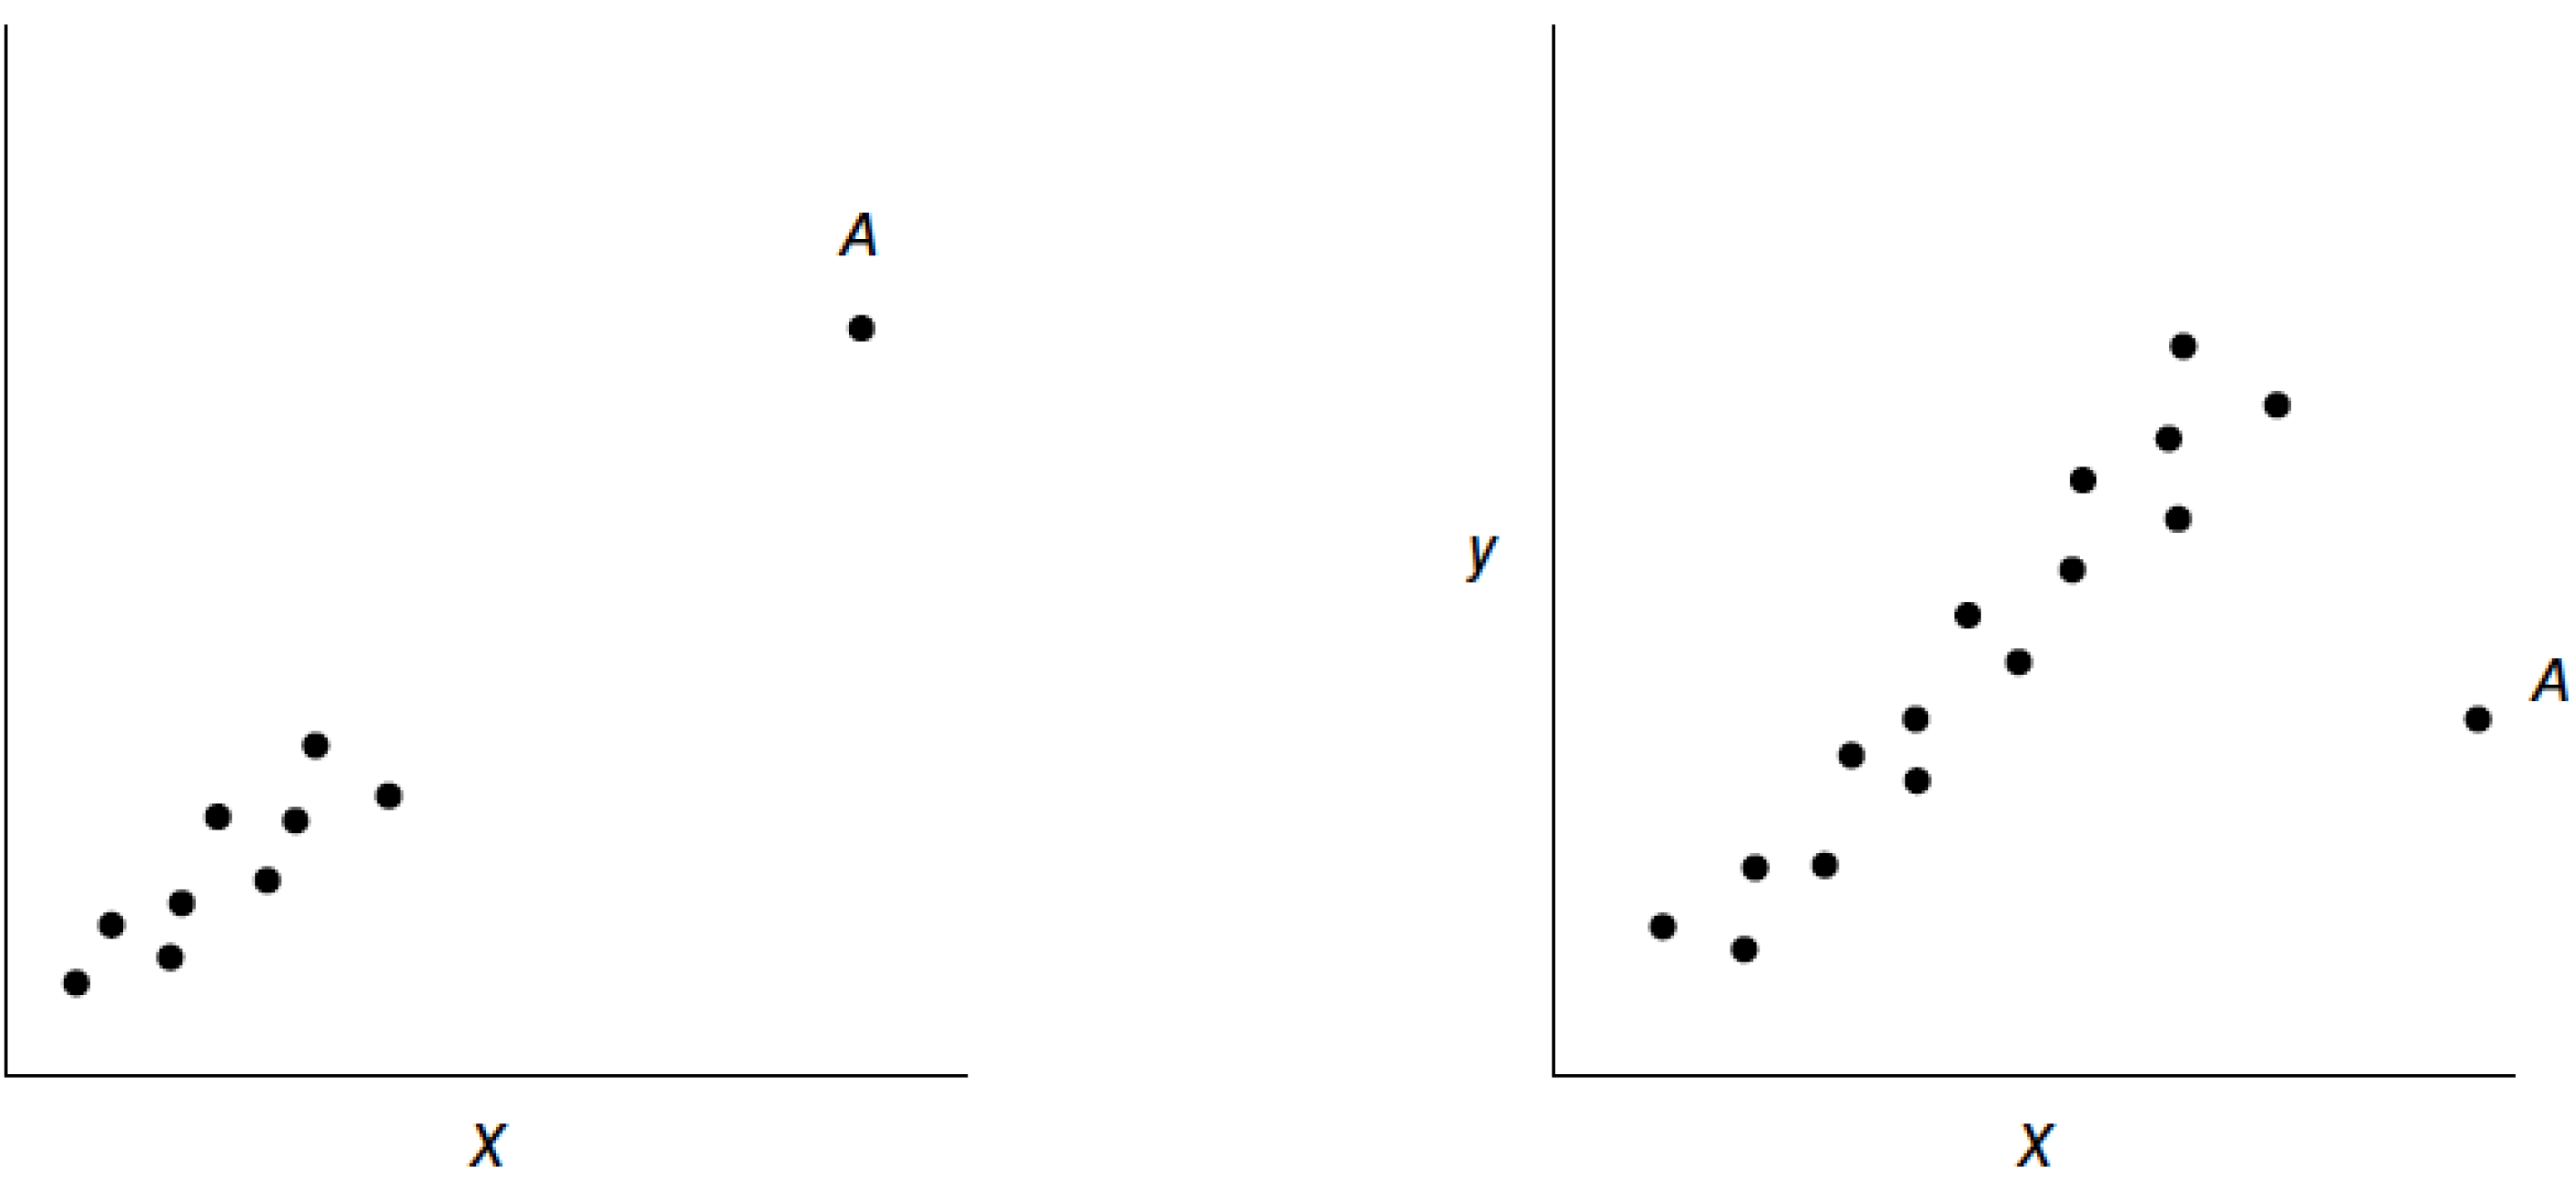
\includegraphics[scale=.22]{figs8/Leverage_Influence.png} 


\end{frame}




\begin{frame}{  Cook's Distance to Detect Influential Points }
\qBrd[4.5in]{gray!30}{ \sqBullet{orange} { Standardized Residual residual:} \tiny   $\HLTY{\HLTW{z_i} := \frac{\hat{Y}_i-Y_i}{\hat{\sigma} }}$
{\tiny: Based on the linear regression assumptions, we might expect the $z_i$'s to resemble a sample from a N(0, 1) distribution.}
}\\
\vspace{.01in}

\qBrd[4.5in]{gray!30}{ \sqBullet{violet}  { Studentized Residual:} It is defined to be  \tiny $\HLTY{\HLTW{e_i} := \frac{\hat{Y}_i-Y_i}{\hat{\sigma}\sqrt{ \HLTEQ[lime]{1-h_{_{i,i}} }  }}}$. {\tiny: approximately follows a t
distribution with $n - p$  degrees of freedom (under the standard assumptions of the SLR).  In large data sets (large n), the standardized
and studentized residuals should not differ dramatically.}
}\\
\vspace{.01in}

\qBrd[4.5in]{gray!30}{ \sqBullet{violet} {Cook's Distance:} \tiny $$\HLTY{\text{CD}_i:= \frac{\HLTW{e_i^2} }{p} \frac{h_{_{i,i}} }{1-h_{_{i,i}} }} .$$
}

\vspace{.1in}
\qBrd[4.5in]{green!30}{
{\bf 
It is suggested to examine the cases with $\text{CD}_i > 0.5$ and that
cases with $\text{CD}_i > 1$ can be highly influential. }}
\end{frame}



%
%\begin{frame}{  Leverage and Influence }
%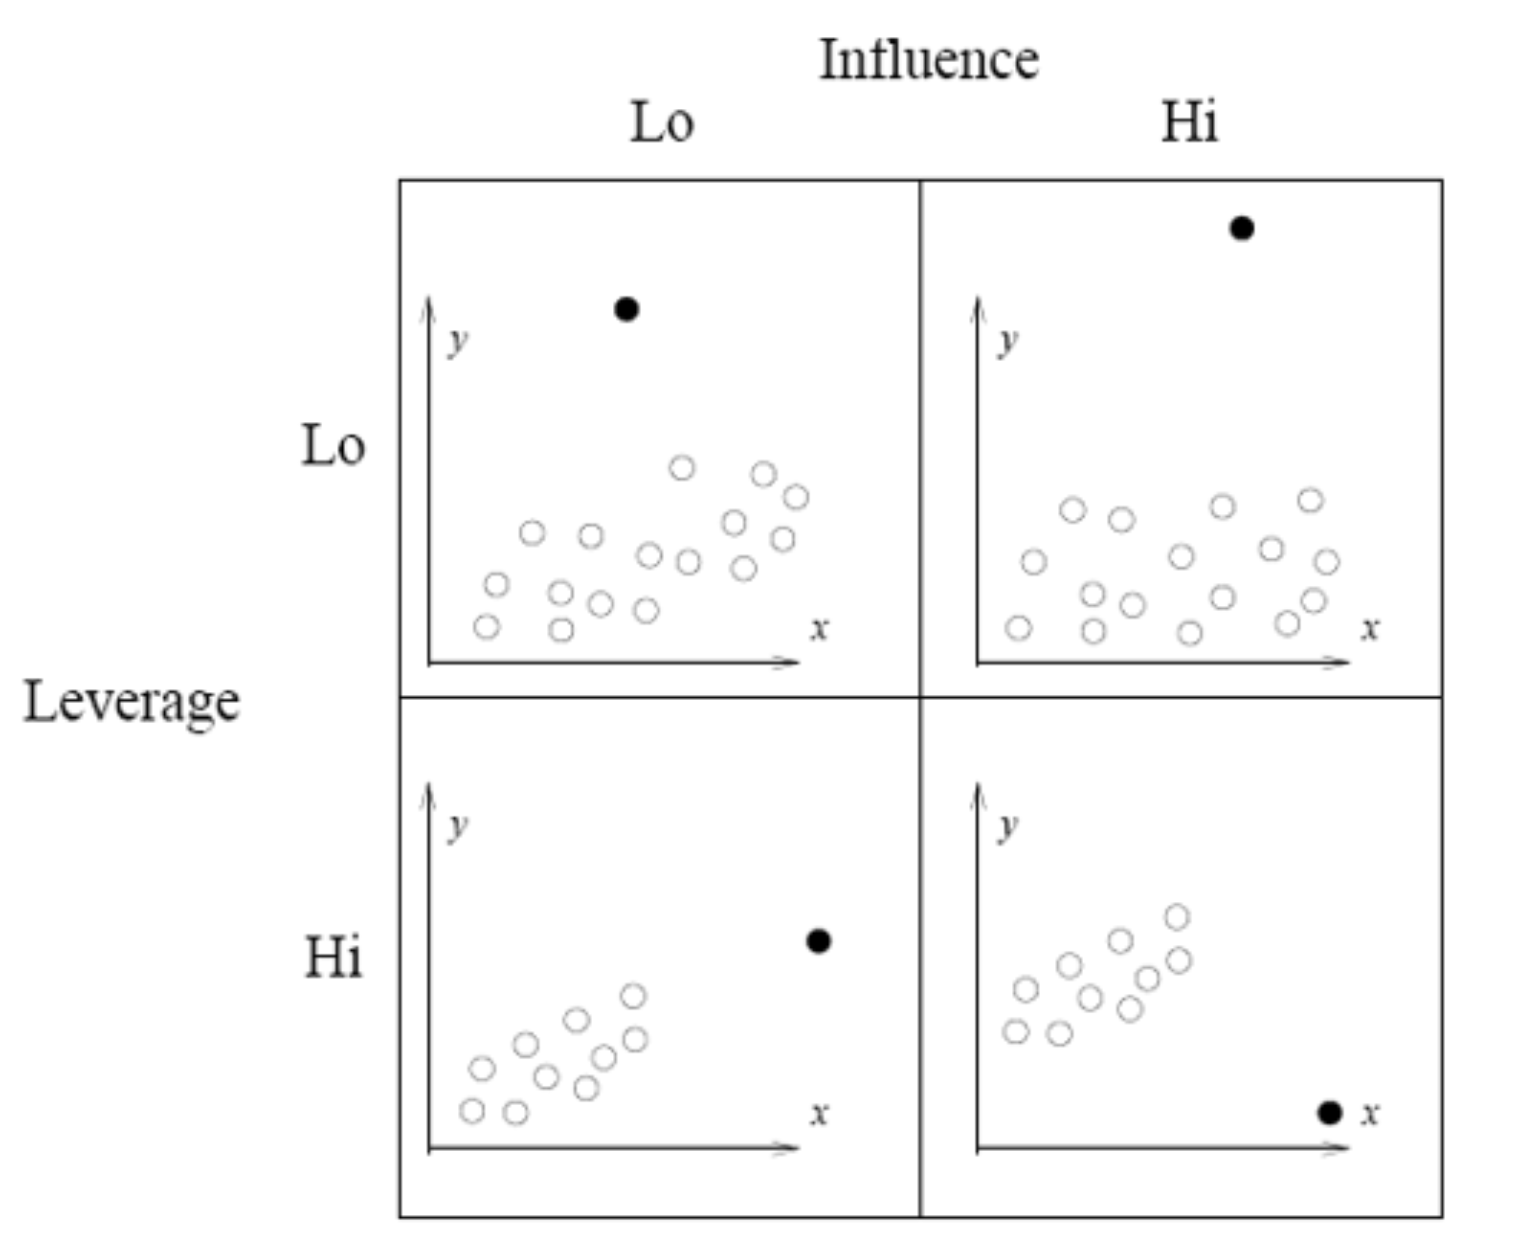
\includegraphics[scale=.35]{figs8/Inf_lev.png} 
%
%
%\end{frame}






\TransitionFrame[antiquebrass]{\Large Residual  Plots}


\begin{frame}{ A Typical Desirable Residual Plot   }
\qBrd{blue!30}{{\bf Residual Plot:} Graph of Residuals against Predictor variable or
against the fitted values is helpful to see if the
variance of error terms are constant. 
}
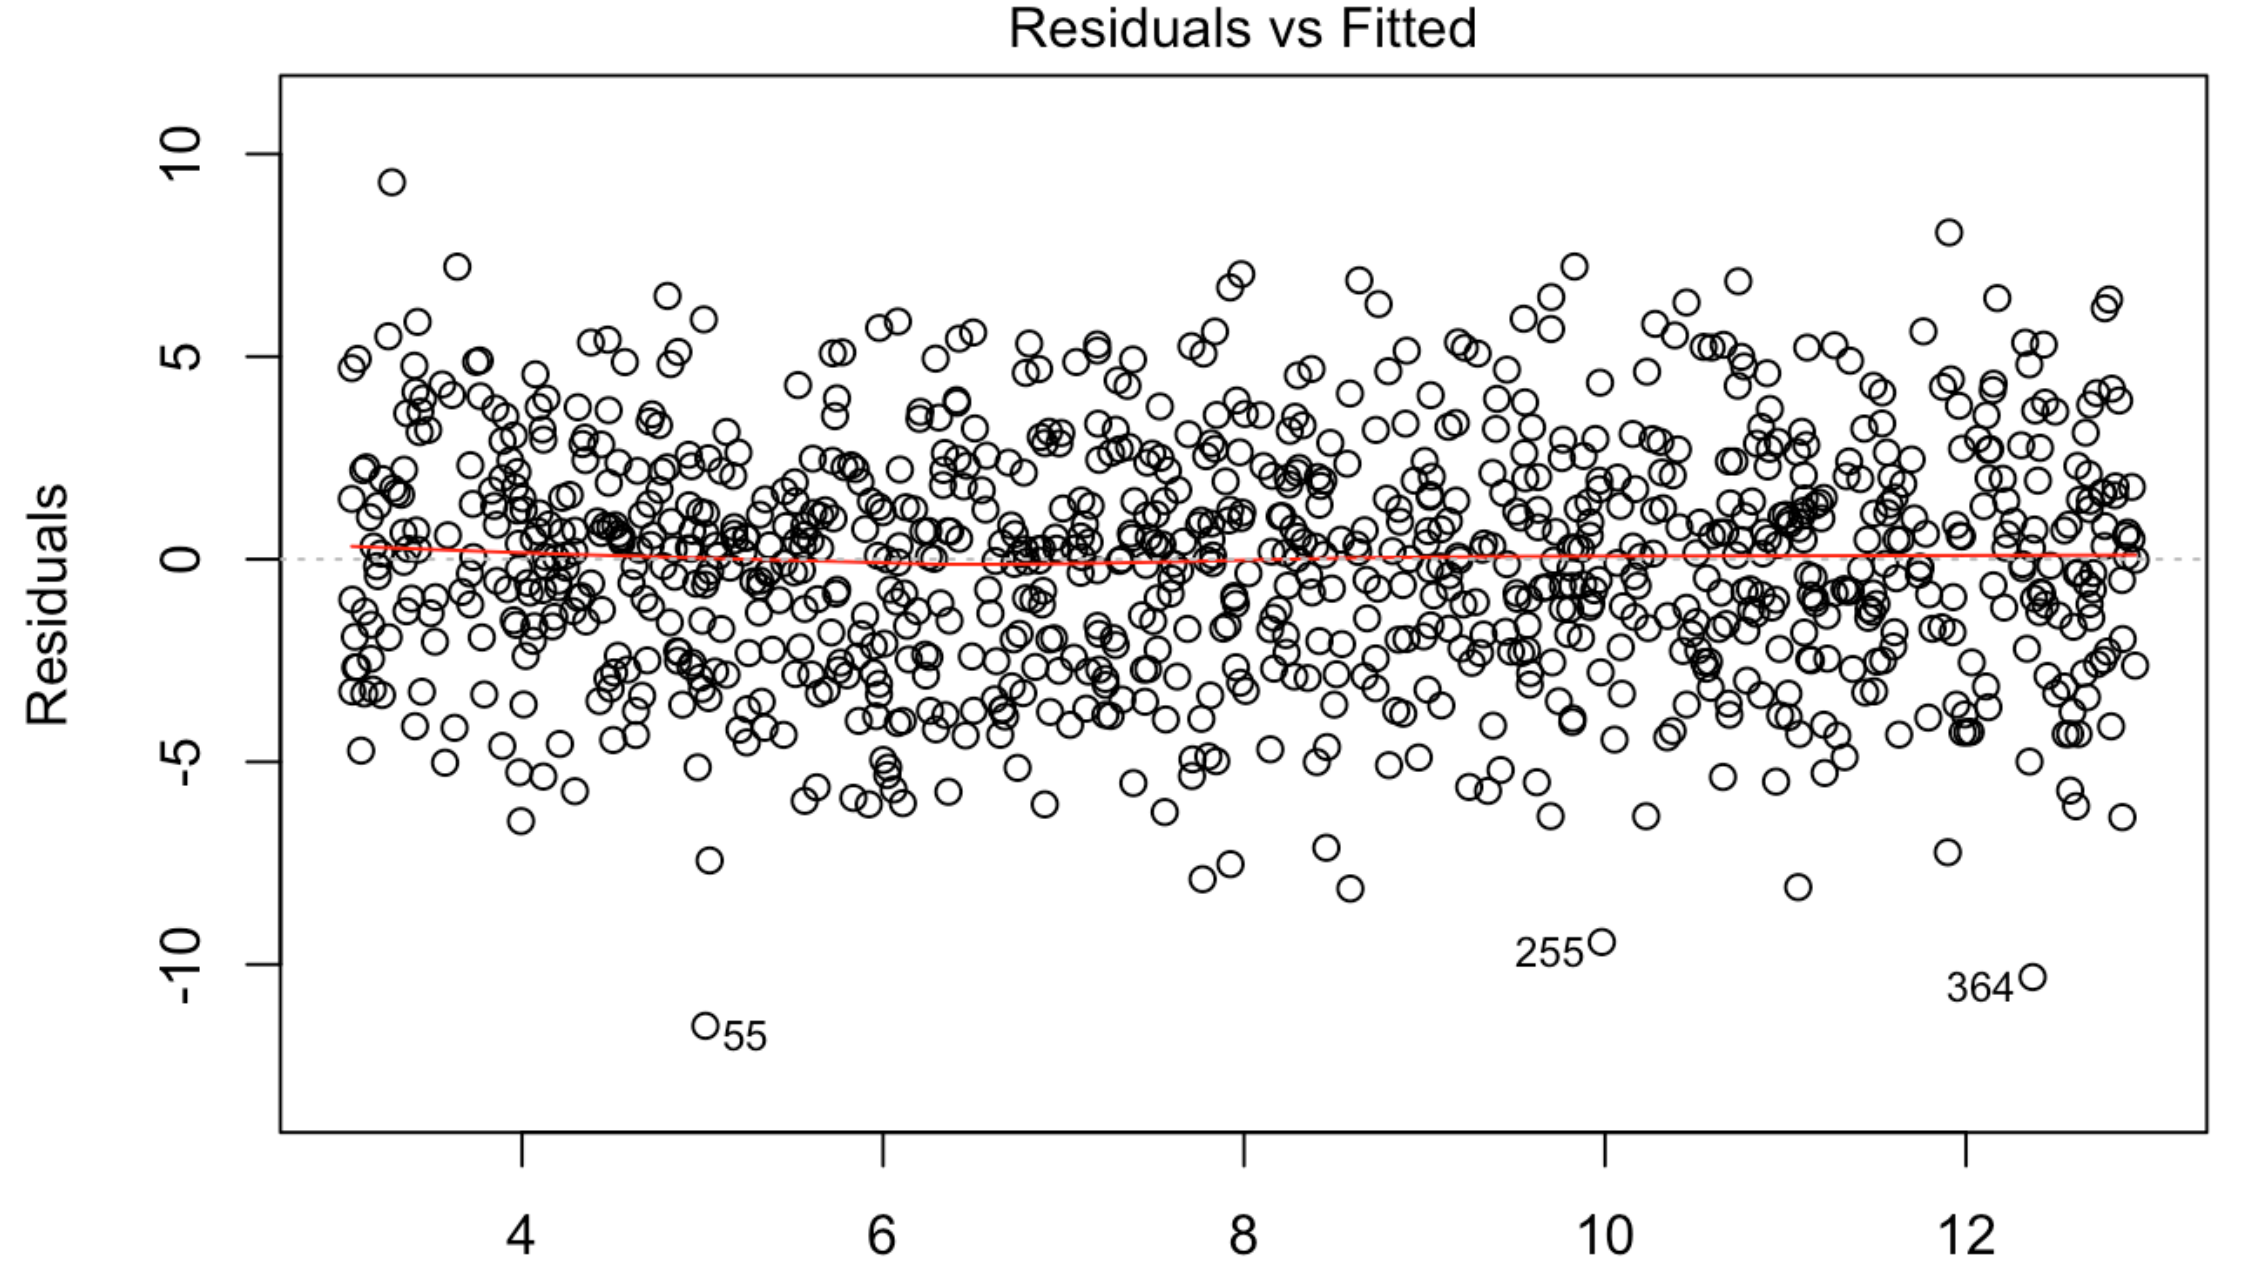
\includegraphics[scale=.3]{figs8/IdealResidual.png} 


\end{frame}


\begin{frame}{   Residual  Plots }

\qBrd[4.6in]{violet!30}{ 
\sqBullet{violet}The plots of the residuals, Studentized Residual and Standardized residuals can be utilized to visually identify  key insights, not only  in identifying influential points, but also many additional information. regarding the regression diagnostics. }
\end{frame}










\TransitionFrame[antiquebrass]{\Large Detection for Lack of Normality of Residuals:\\  Shapiro-Wilk's Test for Residuals}


\begin{frame}{ Normal Q-Q Plot }

\qBrd[4.5in]{blue!30}{  {\bf Normal Q-Q Plot:} Theoretical quantiles (percentiles) from the standard normal distribution are plotted against the empirical quantiles of the standardized residuals. 
}\\
\vspace{.2in}

\qBrd[4.5in]{green!30}{ In ideal scenario, when there is no model assumptions violation on normality of the residuals,  all the points on a Normal Q-Q plot for the standardized residuals should be on the (very close to the) X=Y straight line.
}\\


\end{frame}





\begin{frame}{  Examples: Q-Q Plots  }
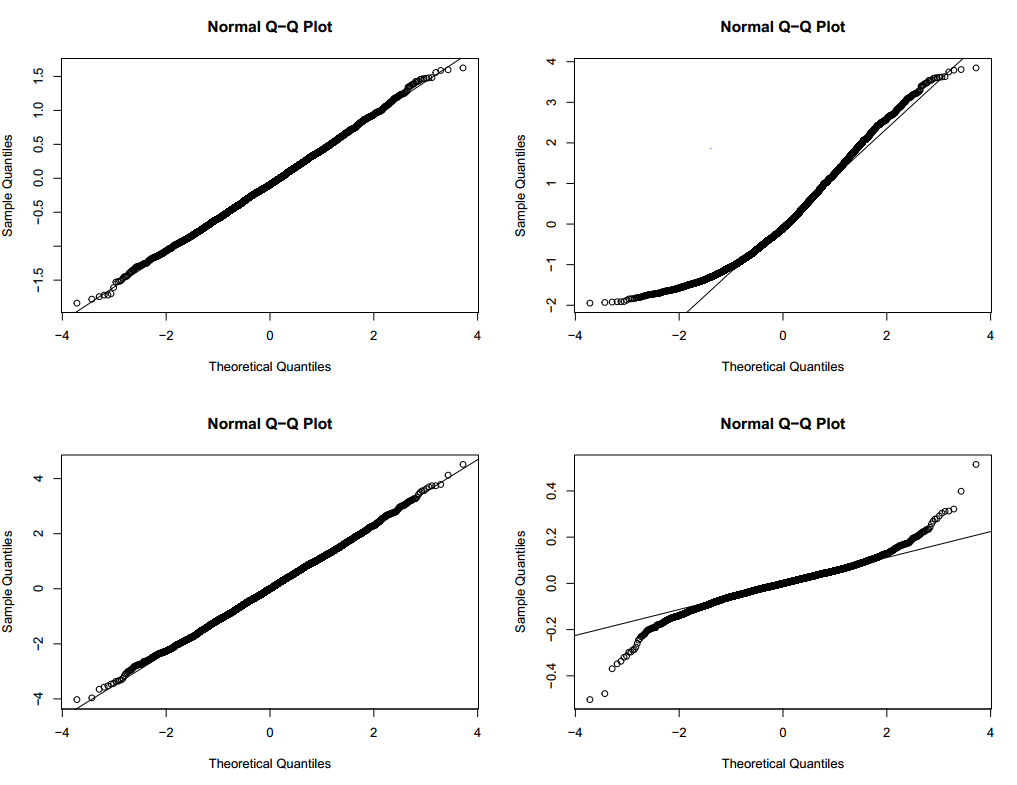
\includegraphics[scale=.3]{figs8/qq_examples.png} 


\end{frame}



\begin{frame}{  Statistical Test of Normality for Residuals: Shapiro-Wilk test  }

\begin{center}
\qBrd{blue!30}{
It tests for whether the errors/residuals are Normally distributed or nor. 
\vspace{-.2in} \begin{center}
\qBrd[2in]{slateblue!50}{$H_0: \text{\tiny Residuals are Normaly Distributed}\\ \text{ vs } \\H_1: \text{ \tiny Residuals are not Normaly Distributed } \vspace{-.01in}$}
\end{center}
}
%\qBrd[4.5in]{gray!30}{ \tiny Define: $e^{*}_{i}:= \hat{Y}_i - Y_i.$ .  Let $e^{*}_{(1)}< e^{*}_{(2)} < \ldots < e^{*}_{(n)}$ are the ordered values of residuals.  }
%\qbx{gray!40}{ $$Test Statistic= \DBX{W= \frac{\sum_{i=1}^{n} a_ie^{*}_{(i)} }{ \sum_{i=1}^{n} \left( e^*_i - \bar{e}^* \right)^2} \text{  where } \bar{e}^* } = \frac{1}{n}\sum{e^*_i}. $$
%}
%\\
%
%\vspace{-.2in}
%\qBrd[4.5in]{slateblue!50}{ $a_1, a_2, \ldots, a_n$ are appropriately chosen numbers related to the joint distribution of n ordered standard normal random variables.  {\tiny Specifically ${\bf a}:= \frac{m^T V^{-1}}{\vert m^T V^{-1}\vert }$}  }\\


\end{center}


\end{frame}

%
%\begin{frame}{  Statistical Test of Normality for Residuals: Shapiro-Wilk test  }
%
%\begin{center}
%\qBrd{blue!30}{
%It tests for whether the errors/residuals are Normally distributed or nor. 
%\vspace{-.2in} \begin{center}
%\qBrd[2in]{slateblue!50}{$H_0: \text{\tiny Residuals are Normaly Distributed}\\ \text{ vs } \\H_1: \text{ \tiny Residuals are not Normaly Distributed } \vspace{-.01in}$}
%\end{center}
%}
%\qBrd[4.5in]{teal!30}{ Define: $e^{*}_{i}:= \hat{Y}_i - Y_i.$ .  Let $e^{*}_{(1)}< e^{*}_{(2)} < \ldots < e^{*}_{(n)}$ are the ordered values of residuals.  }
%\qbx{violet!40}{ $$Test Statistic= \DBX{W= \frac{\sum_{i=1}^{n} a_ie^{*}_{(i)} }{ \sum_{i=1}^{n} \left( e^*_i - \bar{e}^* \right)^2} \text{  where } \bar{e}^* } = \frac{1}{n}\sum{e^*_i}. $$
%}
%\\
%
%\qBrd[4.5in]{slateblue!50}{ $a_1, a_2, \ldots, a_n$ are appropriately chosen numbers related to the joint distribution of n ordered standard normal random variables.  {\tiny Specifically ${\bf a}:= \frac{m^T V^{-1}}{\vert m^T V^{-1}\vert }$ where m, V be the mean and variance of the n ordered standard normal random variables.  }   }\\
%
%
%
%\end{center}
%
%
%\end{frame}
%





\begin{frame}{  Statistical Test of Normality for Residuals: Shapiro-Wilk test  }

\begin{center}
\qBrd{blue!30}{
It tests for whether the errors/residuals are Normally distributed or nor. 
\vspace{-.2in} \begin{center}
\qBrd[2in]{slateblue!50}{$H_0: \text{\tiny Residuals are Normaly Distributed}\\ \text{ vs } \\H_1: \text{ \tiny Residuals are not Normaly Distributed } \vspace{-.01in}$}
\end{center}
}\\
\vspace{.1in}
\qBrd[4.5in]{gray!50}{The test statistic is Denoted as W. $0<W\leq 1$.  $W$ is a fraction.  } \\
\vspace{.1in}


\qBrd[4.5in]{gray!50}{ Decision: We have strong statistical evidence to Reject the Null Hypothesis if the corresponding p-value is less than .05.    }
 \\
\vspace{.1in}

\qBrd[4.5in]{green!50}{ If Assumption of normality are true : the  p-value is {\bf  more then  .05} then there is no statistical evidence to believe that the residuals are not Normally distributed.    }

\end{center}


\end{frame}

\definecolor{airforceblue}{rgb}{0.36, 0.54, 0.66}
\TransitionFrame[airforceblue]{\Large A Possible Remedy to Deal with Non-Normality of the Residuals.    }




\begin{frame}{  Box-Cox Power  Transformation of the Responses }

The power transformation is parametrized by $\lambda $ (a real value can be positive negative or zero.)
\begin{center}
\qBrd{blue!30}{\begin{center}
\DBX{ \tilde{Y} = 
\begin{cases}
\log(Y) & \text{ if } \lambda=0\\
\frac{Y^{\lambda}-1}{\lambda} &\text{ if } \lambda\neq 0\\
\end{cases} }\end{center}
}\\
\vspace{.1in}
\qBrd[4.5in]{violet!50}{\sqBullet{violet}Optimal $\lambda$ is often estimated by a cross validation procedure.  Standard Statistical software typically provide a procedure to identify its optimal value. } \\
\vspace{.1in}
\qBrd[4.5in]{lime!50}{ \sqBullet{green} Box-Cox Transformation may resolve the issues due to the non normality of the residuals and heteroscedasticity. } \\
\vspace{.1in}


\end{center}


\end{frame}


\definecolor{armygreen}{rgb}{0.29, 0.33, 0.13}

\TransitionFrame[armygreen]{\Large  Detection of  heteroscedasticity (Non constant $\sigma^2$)}



\begin{frame}{ Identification of non-constant Error Variance   }
\qBrd{blue!30}{{\bf Residual Plot:} Graph of Residuals against Predictor variable or
against the fitted values is helpful to see if the
variance of error terms are constant. 
}
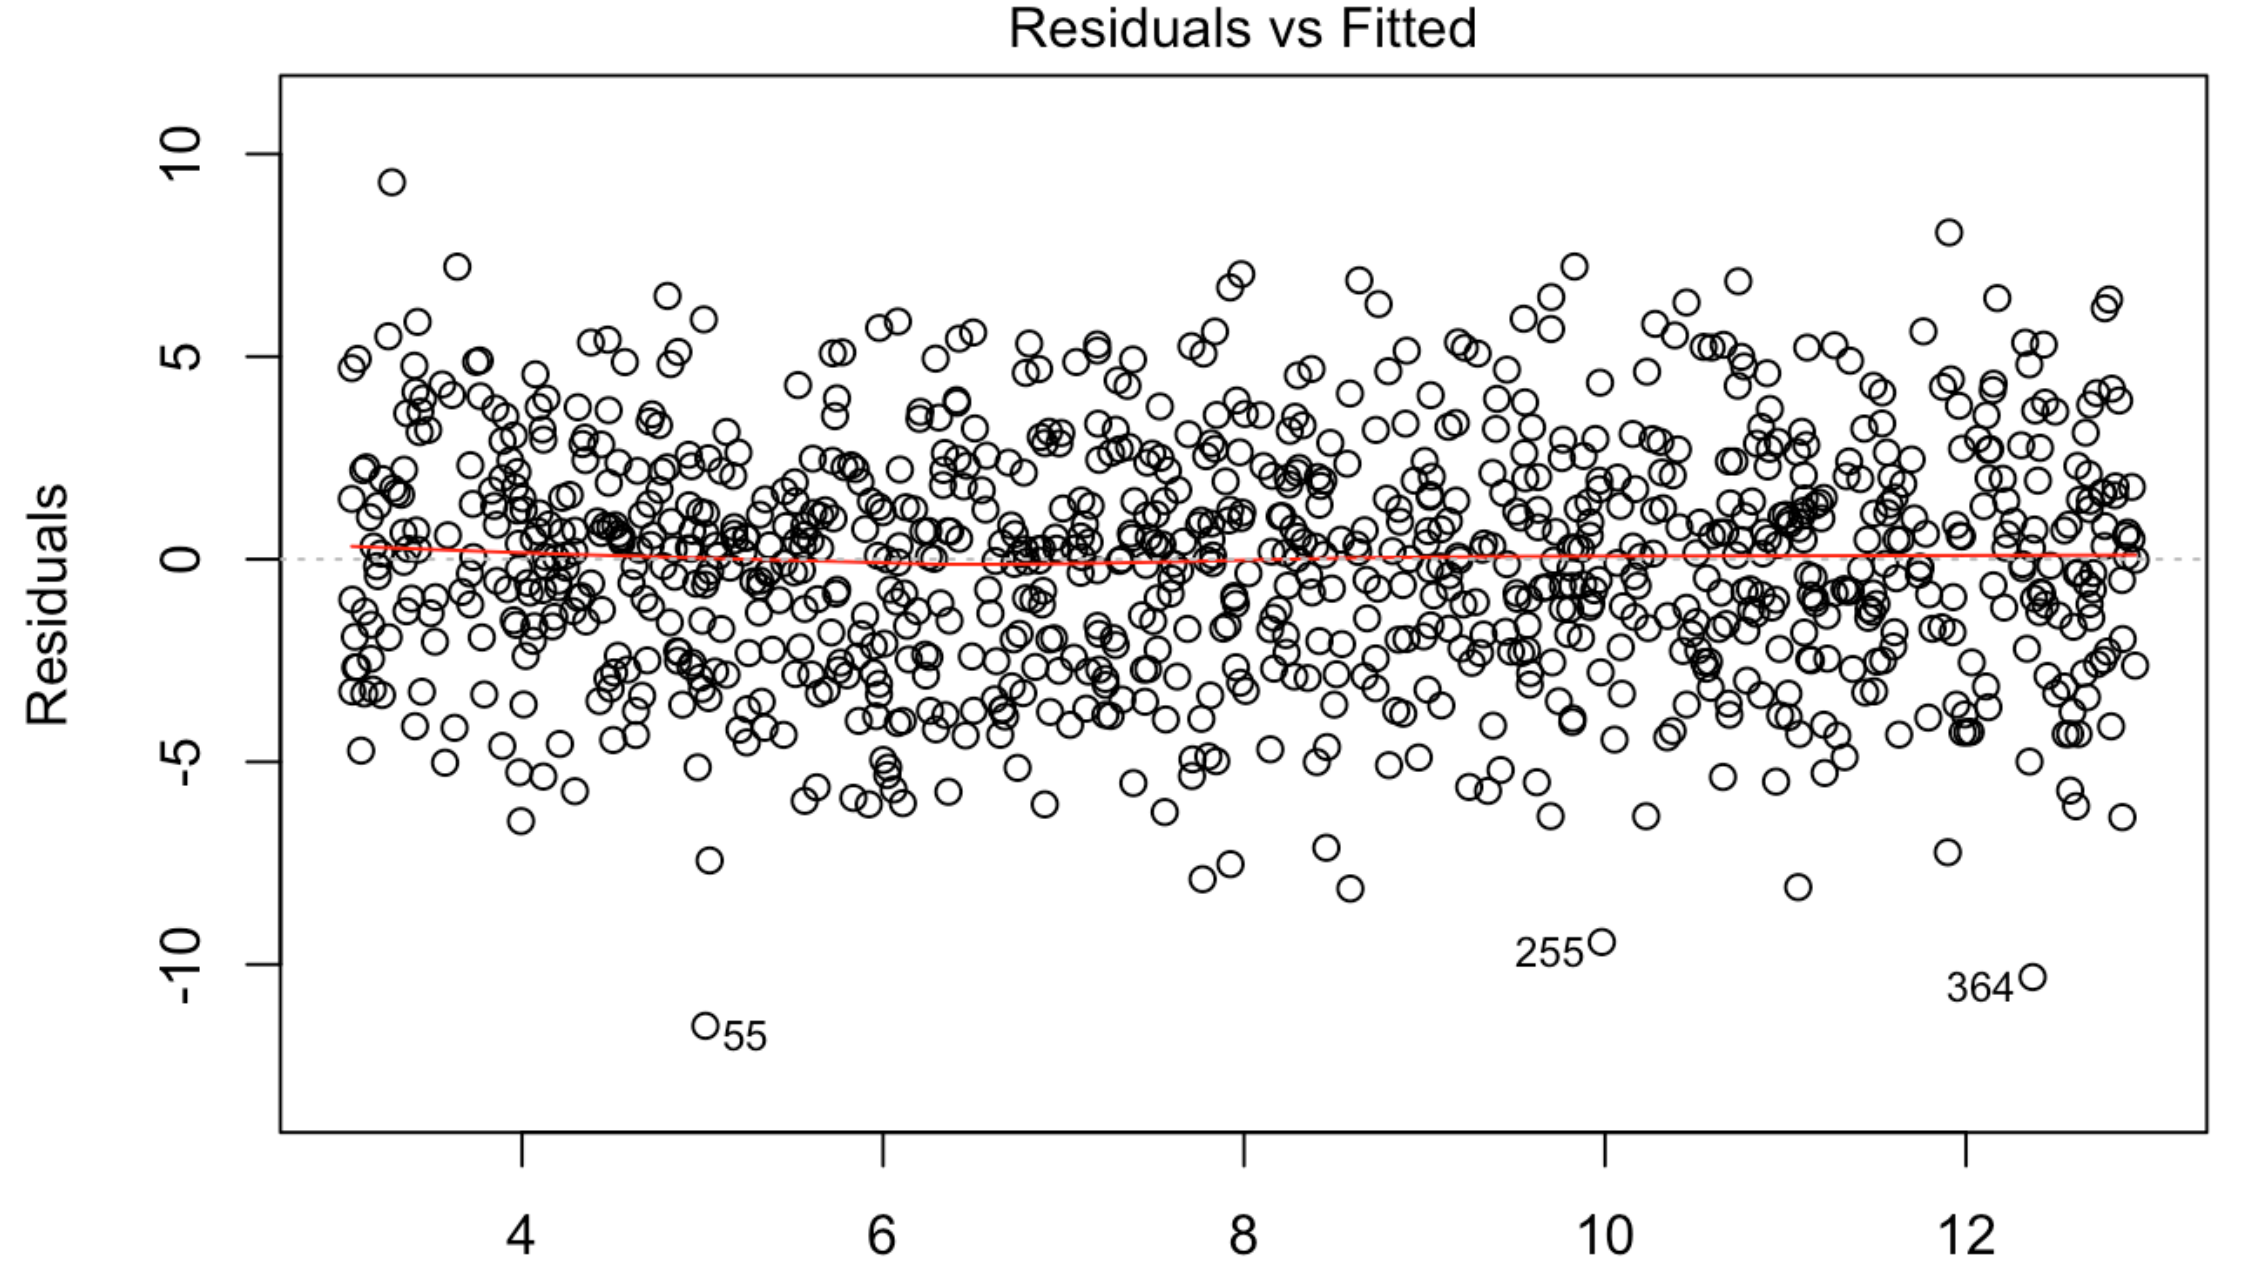
\includegraphics[scale=.3]{figs8/IdealResidual.png} 


\end{frame}



\begin{frame}{ Identification of non-constant Error Variance   }
\qBrd{blue!30}{{\bf Residual Plot:}  Variability of the residuals appears to be increasing.
}
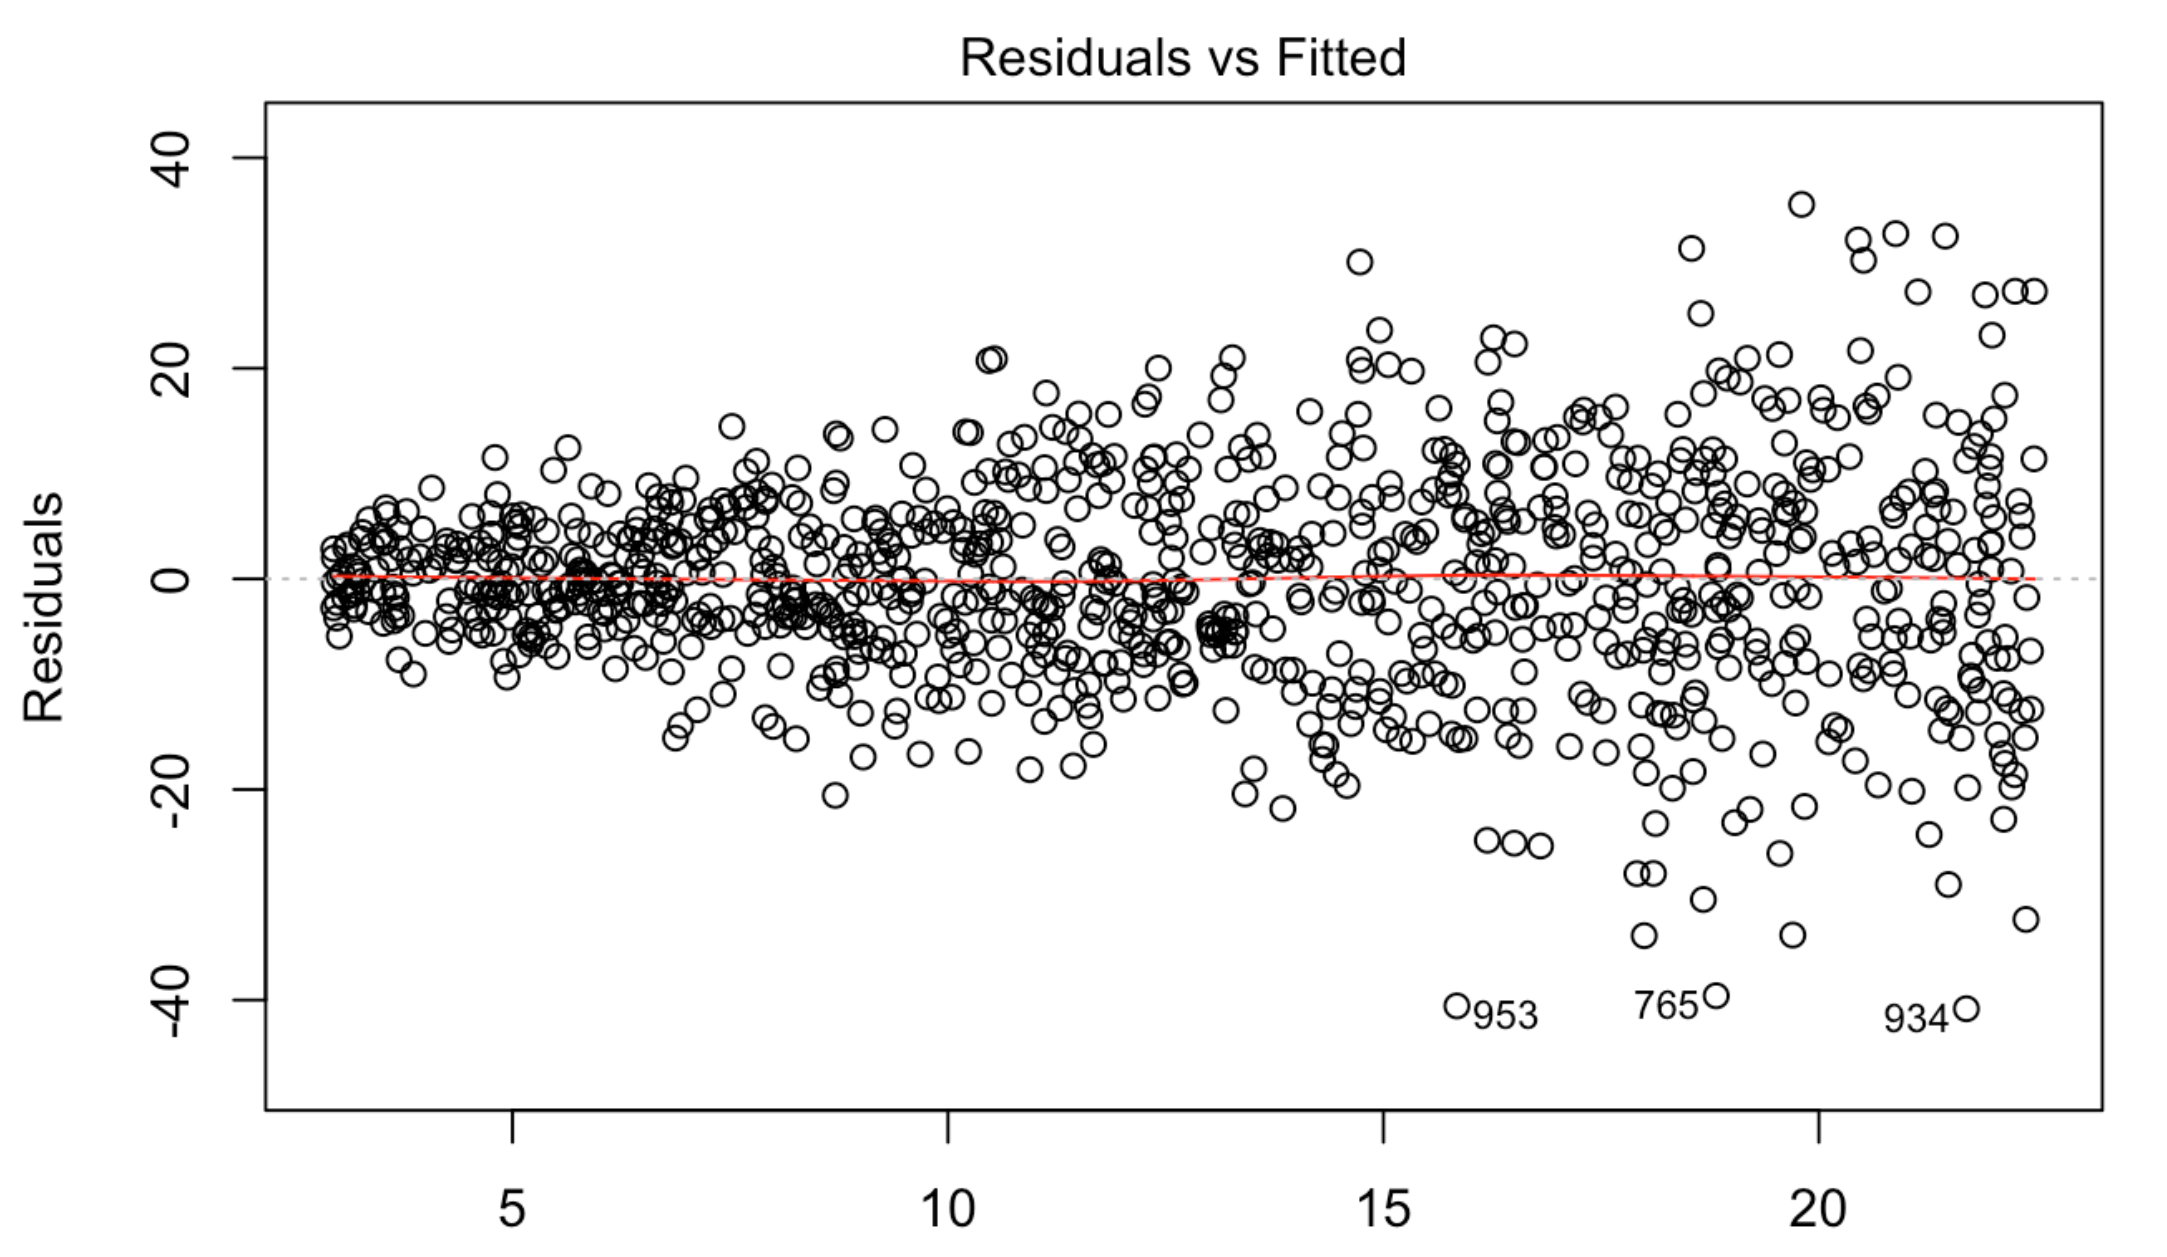
\includegraphics[scale=.3]{figs8/varIncrease.png} 


\end{frame}






\begin{frame}
\qBrd{airforceblue!50}{ \sqBullet{airforceblue} A Possible remedy to deal with non constant variability is to utilize weighted Least Square. }

\qBrd{green!20}{ \sqBullet{airforceblue} Use appropriate transformation on the Responses (Y).}
\end{frame}








\TransitionFrame[antiquebrass]{\Large  Detection of Correlated Model Errors ($\varepsilon_i$): \\ Durbin-Watson Test}



\begin{frame}{ Identification of Non Linearity  }
\qBrd{blue!30}{{\bf Residual Plot:}  Violation of the Linearity Assumption. The errors are not statistically independent/uncorrelated.  There seem to be  a seasonality.
}
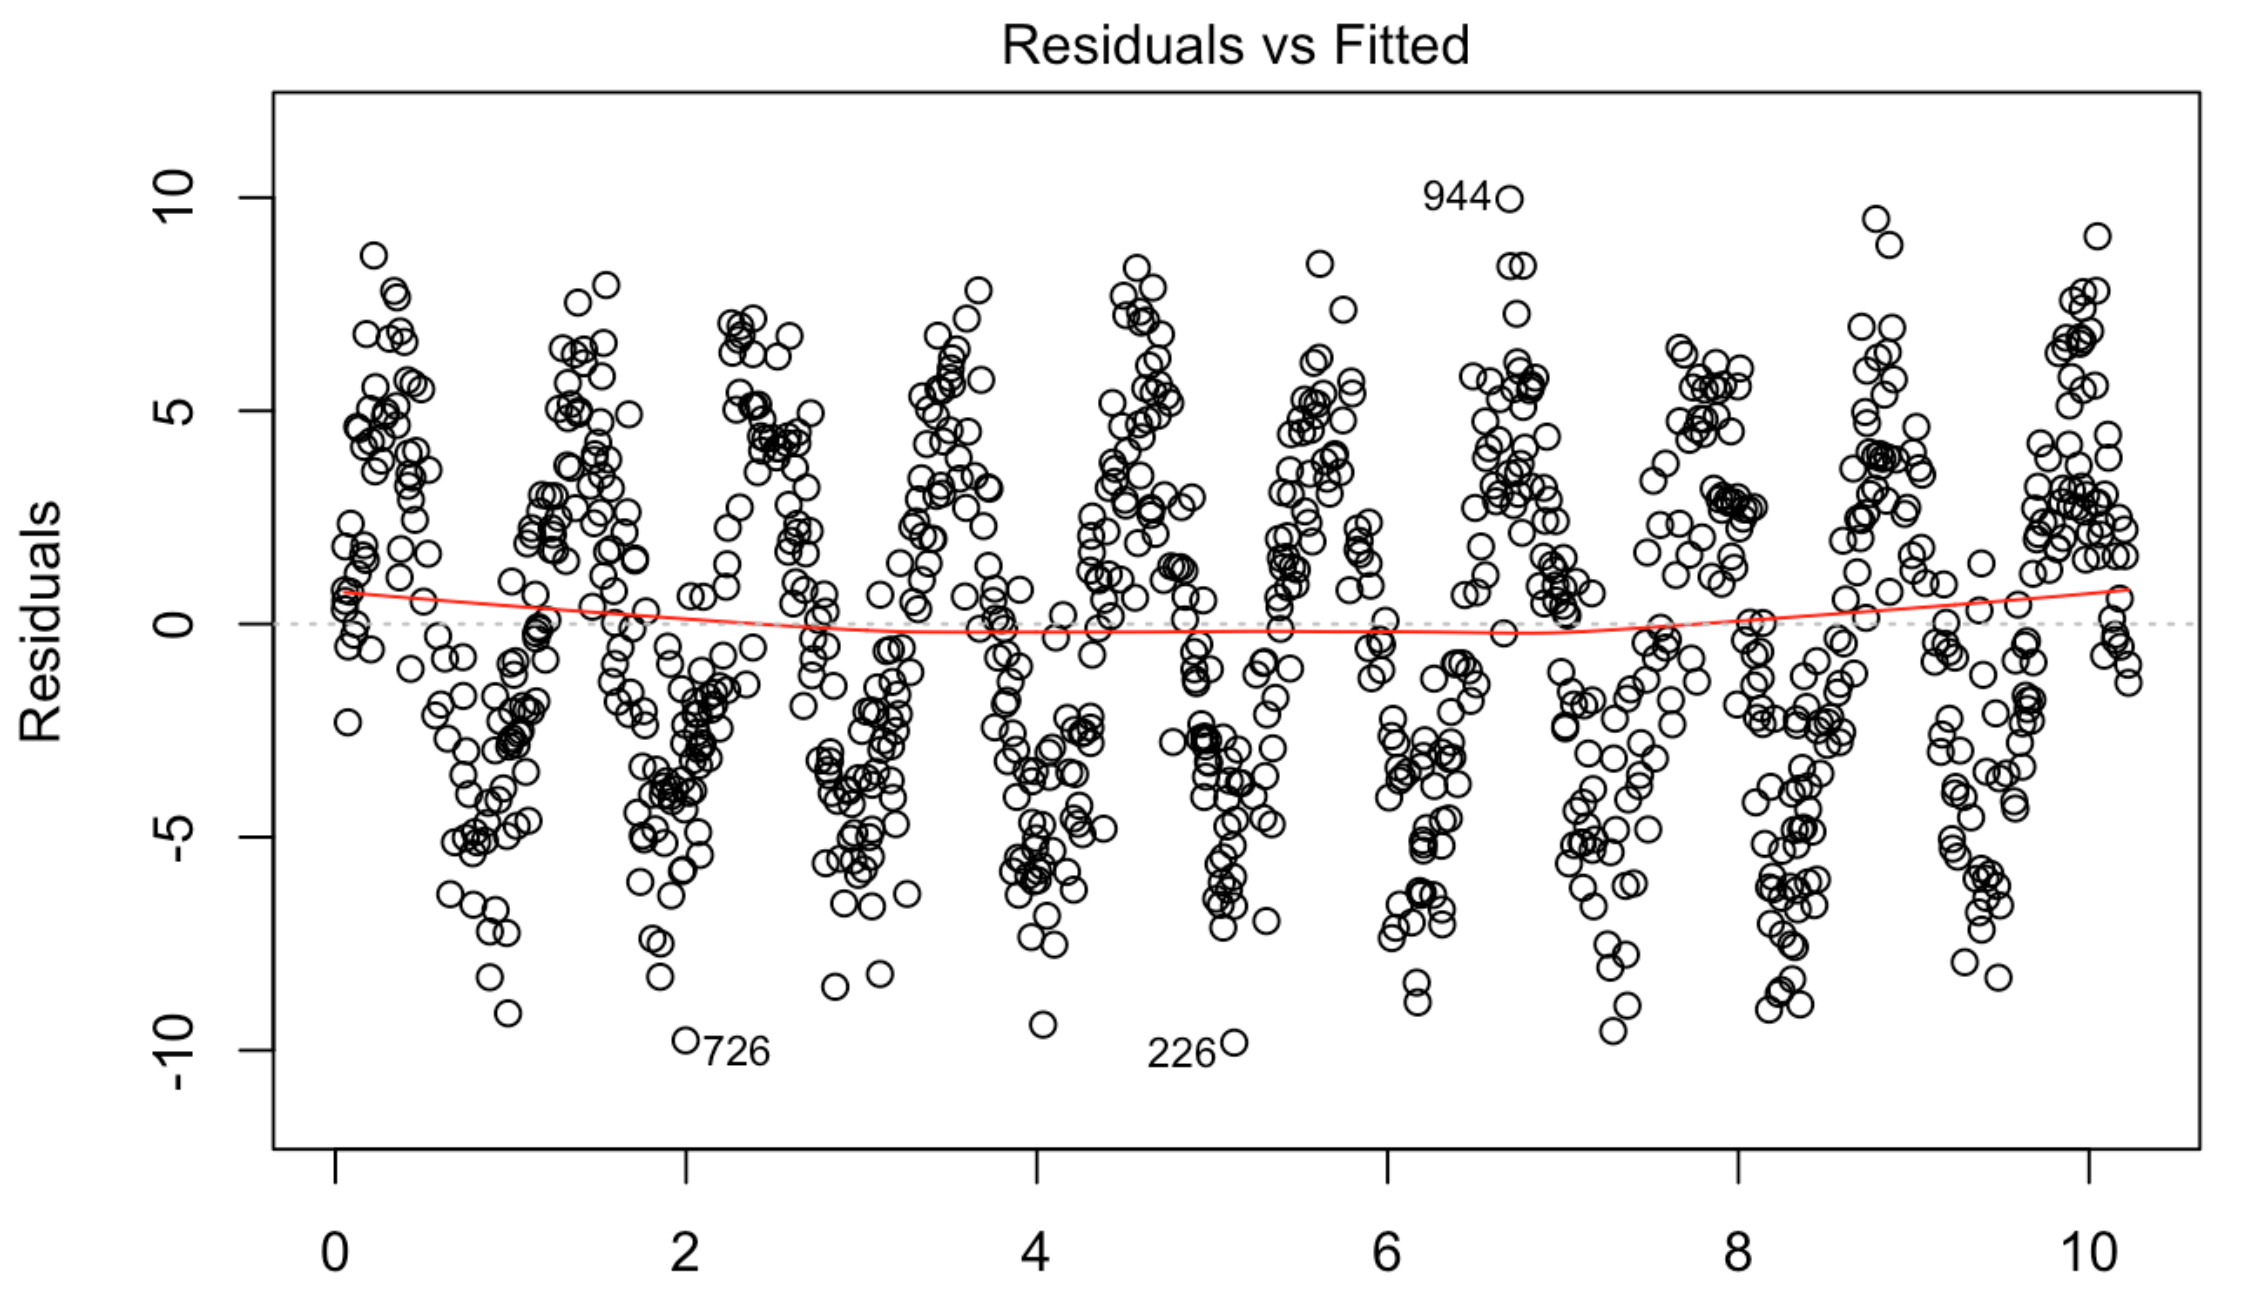
\includegraphics[scale=.28]{figs8/Seasonal.png} 


\end{frame}

\begin{frame}{ Darbin Watson Test (DW Test) for identifying Correlated Model Errors }
\vspace{-.05in}
\begin{center}
\qBrd{blue!30}{
It tests for whether the errors/residuals are auto-correlated or not.  Let $\rho$ denotes the lag 1 auto correlation between the errors.   i.e.  If $\text{corr}( \varepsilon_i,  \varepsilon_{i-1})= \rho$ then it tests for\\
\vspace{-.2in} \begin{center}
\qBrd[3in]{slateblue!50}{$$H_0: \rho= 0 \text{ vs } H_1: \rho\neq 0 \vspace{-.1in}$$}
\end{center}
}

\qBrd[2in]{olive!50}{ \tiny Define: $e^{*}_{i}:= \hat{Y}_i - Y_i.$ }
\qbx{violet!40}{ \tiny $Test Statistic= d= \frac{\sum_{i=1}^n\left(e^{*}_{i}- e^{*}_{i-1}\right)^2}{\sum_{i=1}^n{e^{*}}^2}$
}

\vspace{-.1in}
\qBrd[4.5in]{gray!50}{ Reject Null Hypothesis if $d$ is large or small.  `significantly large' value of d indicates negative correlation,  `significantly small' values of d is indicative of positive correlation   }



\qBrd[4.5in]{green!50}{ Assumption are met (errors are not correlated ): If the corresponding p-value of the test is LARGER than .05 }



\end{center}
\end{frame}

\begin{frame}
\qBrd{airforceblue!50}{ \sqBullet{airforceblue} A Possible remedy is to use  utilize Time series models such as AR, ARMA, ARIMA, GARCH model. Uf there is seasonality in the model try to include some periodic function along with the linear functions.  }
\end{frame}



\TransitionFrame[antiquebrass]{\Huge Thank You}


\end{document}
